\documentclass[12pt]{extarticle}
\usepackage{geometry}
\geometry{
a4paper,
total={170mm,257mm},
left=20mm,
top=20mm,
headheight=12pt
}

%\usepackage[parfill]{parskip} % Activate to begin paragraphs with an empty line rather than an indent
\usepackage{graphicx} % Use pdf, png, jpg, or eps§ with pdflatex; use eps in DVI mode
% TeX will automatically convert eps --> pdf in pdflatex
\usepackage[labelfont=bf]{caption}
\usepackage{float}

\usepackage{amssymb,amsmath,amsthm}
\usepackage{commath}
\usepackage[hyphens]{url}
\usepackage[dvipsnames]{xcolor}
\usepackage[unicode=true,colorlinks=true,urlcolor=CadetBlue,citecolor=black,linkcolor=black]{hyperref}
\PassOptionsToPackage{hyphens}{url} % url is loaded by hyperref
\usepackage{authblk}
\usepackage{longtable}
\usepackage{multirow}
\usepackage{booktabs}
\usepackage{lipsum}  
\usepackage[title,page]{appendix}
\usepackage{chngcntr}
%\usepackage{end float}
\usepackage{cleveref}
 \usepackage{subcaption}

%SetFonts
% newtxtext+newtxmath
\usepackage{newtxtext} %loads helv for ss, txtt for tt
\usepackage{amsmath}
\usepackage[bigdelims]{newtxmath}
\usepackage[T1]{fontenc}
\usepackage{textcomp}
%SetFonts

% less space before sections 
% https://tex.stackexchange.com/a/101126
%\usepackage{titlesec}
%\titlespacing*{\section}{0pt}{0.5\baselineskip}{0\baselineskip}
%\titlespacing*{\subsection}{0pt}{0.5\baselineskip}{0\baselineskip}
    
% Species names
%% Meta-Command for defining new species macros
\usepackage{xspace}

\newcommand{\species}[3]{%
  \newcommand{#1}{\gdef#1{\textit{#3}\xspace}\textit{#2}\xspace}}
  \species{\yeast}{Saccharomyces cerevisiae}{S.~cerevisiae}

% line numbers
\usepackage[displaymath, mathlines]{lineno}
\renewcommand\linenumberfont{\normalfont\small\sffamily}
\linenumbers
\modulolinenumbers[2]

% Yoav & Lee commands
\newcommand*{\tr}{^\intercal}
\let\vec\mathbf
\newcommand{\matrx}[1]{{\Big[ \stackrel{}{#1}\Big]}}
\newcommand{\diag}[1]{\mbox{diag}\matrx{#1}}
\newcommand{\goesto}{\rightarrow}
\newcommand{\dspfrac}[2]{\frac{\displaystyle #1}{\displaystyle #2} }
\newtheorem{theorem}{Theorem}
\newtheorem{corollary}{Corollary}
\newtheorem{lemma}{Lemma}
\newtheorem{remark}{Remark}
\newtheorem{result}{Result}
\renewcommand\qedsymbol{} % no square at end of proof
\newcommand{\cl}{\mathbf{L}}
\newcommand{\cj}{\mathbf{J}}
\newcommand{\ci}{\mathbf{I}}
\newcommand{\E}{\mathbf{E}}
\DeclareMathOperator{\sign}{sign}
\renewcommand{\d}[1]{\ensuremath{\operatorname{d}\!{#1}}}

% Remus commands
\newcommand{\x}{{\bf x}}
\renewcommand{\d}{{\rm d}}
\newcommand{\e}{{\rm e}}
\newcommand{\erfc}{{\rm erfc}}
\newcommand{\ii}{{\rm i}}

\newcommand{\tmi}{\tau_0\wedge\tau}
\newcommand{\tma}{\tau_0\vee\tau}
\newcommand{\taua}{\tau_{\rm A}}

% Supplementary
% https://support.authorea.com/en-us/article/how-to-create-an-appendix-section-or-supplementary-information-1g25i5a/
\newcommand{\beginsupplement}{%
      	\setcounter{table}{0}
        \renewcommand{\thetable}{S\arabic{table}}%
        \setcounter{figure}{0}
        \renewcommand{\thefigure}{S\arabic{figure}}%
		\setcounter{equation}{0}
        \renewcommand{\theequation}{A\arabic{equation}}%
}

% autoref
\def\equationautorefname{Eq.}

% NatBib
\usepackage[comma,sort]{natbib}

%%%%%%%%%%%%%%%%%%%%%%%%%%%%%%%%%%%%%%%%%%%%%%%%%%%%%%

% Title page
\title{The role of aneuploidy in the evolution of cancer drug resistance}
% Authors
\renewcommand\Affilfont{\small}

\author[1]{Remus Stana}
\author[2]{Uri Ben-David}
\author[3]{Daniel B. Weissman}
\author[1,*]{Yoav Ram}
\affil[1]{School of Zoology, Faculty of Life Sciences, Tel Aviv University, Tel Aviv, Israel}
\affil[2]{Department of Human Molecular Genetics and Biochemistry, Faculty of Medicine, Tel Aviv University, Tel Aviv, Israel}
\affil[3]{Department of Physics, Emory University, Atlanta, GA}
\affil[*]{Corresponding author: yoav@yoavram.com}
 
%%%%%%%%%%%%%%%%%%%%%%%%%%%%%%%%%%%%%%%%%%
\begin{document}
\maketitle

%%%%%%%%%%%%%%%%%%%%%%%%%%%%%%%%%%%%%%%%%%
\begin{abstract}
%Evolutionary rescue is the process by which a population is able to survive a sudden environmental change which initially causes the population to decline towards extinction. A prime example of evolutionary rescue is the ability of cancer to survive being exposed to various treatments. We are interested in the mechanisms through which a population of cancer cells are able to adapt to chemotherapy, and in particular, the role played by chromosomal instability (aneuploidy). Cancer cells which have aneuploidy are hypothesized to have a higher fitness in an environment altered by anti-cancer drugs as they have incomplete pathways which drugs activate in order to kill the cells. Aneuploidy is highly prevalent in tumors and certain drugs which attempt to combat cancers through increasing chromosomal instability. As a result, the question we wish to answer is how aneuploidy impacts the fate of the population of cancer cells. We propose to model evolutionary rescue with the help of multi-type branching processes to obtain the probability that cancer will survive. Additionally, we will utilize large genomic datasets to asses the effects of aneuploidy on the probability of evolutionary rescue.
\end{abstract}

\newpage
%%%%%%%%%%%%%%%%%%%%%%%%%%%%%%%%%%%%%%
\section*{Introduction}

%%%%%%

% OVERVIEW OF INTRODUCTION:
% - background on CIN in cancer
% - what hasn't been done? (aneuploidy + drug resistance)
% - why is that important?
% - how we tackle this background
% - summary of our analysis
% history of evolutionary rescue literature (that is not specific to cancer) should move to literature, and we should have a clear statement on what we add to that literature. 

% TODO two papers that show aneuploidy provides resistance
% Lukow, Devon A., Erin L. Sausville, Pavit Suri, Narendra Kumar Chunduri, Angela Wieland, Justin Leu, Joan C. Smith, et al. 2021. “Chromosomal Instability Accelerates the Evolution of Resistance to Anti-Cancer Therapies.” Developmental Cell 56 (17): 2427-2439.e4. https://doi.org/10.1016/j.devcel.2021.07.009.
% Rutledge, Samuel D., Temple A. Douglas, Joshua M. Nicholson, Maria Vila-Casadesús, Courtney L. Kantzler, Darawalee Wangsa, Monika Barroso-Vilares, Shiv D. Kale, Elsa Logarinho, and Daniela Cimini. 2016. “Selective Advantage of Trisomic Human Cells Cultured in Non-Standard Conditions.” Scientific Reports 6 (June 2015): 1–12. https://doi.org/10.1038/srep22828.

\paragraph{Aneuploidy in cancer.} Chromosomal instability (CIN) is the mitotic process in which cells suffer from chromosome mis-segregation that leads to aneuploidy, where cells are characterized by structural changes of the chromosomes and copy number alterations \citep{schukken2018cin}.
Interestingly, aberrations in chromosome copy number have been shown to allow cancer cells to survive under stressful conditions such as drug therapy.
Indeed, cancer cells are often likely to be aneuploid, and aneuploidy is associated with poor patient outcomes \citep{ben2020context}.

The role of chromosomal instability (CIN) in the emergence of cancer has been studied extensively in the past decades \citep{michor2005can,christine2018understanding,nowak2002role,pavelka2010dr,komarova2003mutation,zhu2018cellular}.
One hypothesis is that CIN facilitates tumor genesis by accelerating the removal of tumor suppression genes (TSG) and subsequent appearance of cancer. The deletion of tumor suppression genes can happen in two ways: two point mutations deleting both alleles of the TSG (assuming a diploid genotype), or one point mutation and one chromosomal loss event.
Initial theoretical studies have shown that aneuploidy can have a significant role in the deletion of the the tumor suppressing genes when compared to two consecutive point mutations \citep{nowak2002role,komarova2003mutation,michor2005can,komarova2008selective}.
However, when taking into account that the appearance of aneuploidy requires a mutation to trigger CIN, the probability that CIN precedes tumor genesis is highly unlikely.

\paragraph{Evolutionary rescue.} Populations adapted to a certain environment are vulnerable to environmental changes, which might cause extinction of the population. Examples of such environmental changes include climate change, invasive species or the onset of drug therapies. Adaptation is a race against time as the population size decreases in the new environment~\citep{tanaka2022surviving}. 
\emph{Evolutionary rescue} is the process where the population acquires a trait that increases fitness in the new environment such that extinction is averted. It is mathematically equivalent to the problem of crossing of fitness valley \citep{weissman2009rate,weissman2010rate}.
There are three potential ways for a population to survive environmental change: migration to a new habitat similar to the one before the onset of environmental change \citep{cobbold2020should}; adaptation by phenotypic plasticity without genetic modification \citep{carja2019evolutionary,carja2017evolutionary,levien2021non}; and adaptation through genetic modifications, e.g., mutation \citep{uecker2014evolutionary,uecker2016role,uecker2011fixation}.

Models of evolutionary rescue usually assume that the fitness of the wildtype and mutant are homogeneous in time. An exception was given by \citet{marrec2020adapt}, who modeled the fitness of the wildtype and mutant as time dependent. Additionally, \citet{uecker2011fixation} investigated the probability of fixation of a beneficial mutation in a variable environment with arbitrary time-dependent selection coefficient and population size.
Most models focus on the probability that at least one mutation rescues the population. How multiple mutations contribute to the survival of the population is less explored, but \citet{wilson2017soft} have shown that evolutionary rescue is significantly enhanced by soft selective sweeps when multiple mutations contribute. 
Evolutionary rescue that requires two successive mutations has been investigated using diffusion approximation by \citet{martin2013probability}.

%%%%%%%%%%%%%%%%%%%%%%%%%%%%%%%%%%%%%%%%%%
\section*{Methods}
\subsection*{Evolutionary model}

We follow the number of cancer cells that have one of three different genotypes at time $t$: wildtype, $w_t$; aneuploid, $a_t$; and mutant, $m_t$. 
These cells divide and die with rates $\lambda_k$ and $\mu_k$ (for $k=w, a, m$).
The difference between the division and death rate is $\Delta_k = \lambda_k-\mu_k$.
We assume the population of cells is under a strong stress, such as drug therapy, to which the wildtype genotype is susceptible and therefore $\Delta_w<0$, whereas the mutant is resistant to the stress, $\Delta_m>0$.
We analyze three scenarios: in the first, aneuploid cells are partially resistant, $\Delta_m>\Delta_a>0$; in the second, aneuploid cells are tolerant, $0>\Delta_a>\Delta_w$ \citep[see][for the distinction between susceptible, resistant, and tolerant]{brauner2016distinguishing}; in the third, aneuploid cells are non-growing or "barely growing", that is, either slightly tolerant or slightly resistant, such that $\Delta_a \approx 0$, in a sense that we will make more precise.
Wildtype cells may missegregate to become aneuploids at rate $u$. Both aneuploid and wildtype cells may mutate to become mutants at rate $v$ (\Cref{figureAneuploidy}). 

%Thus, the changes in the number of each cell type is described by 
%\begin{equation}
%\begin{aligned}
%w_t&\rightarrow w_t+1:\quad \lambda_ww_t,\\
%w_t&\rightarrow w_t-1:\quad \left(\mu_w+u+v\right)w_t,\\
%a_t&\rightarrow a_t+1:\quad \lambda_aa_t+uw_t,\\
%a_t&\rightarrow a_t-1:\quad \left(\mu_a+v\right)a_t,\\
%m_t&\rightarrow m_t+1:\quad \lambda_am_t+va_t+vm_t,\\
%m_t&\rightarrow m_t-1:\quad \mu_am_t.
%\end{aligned}
%\end{equation}

%%%%%%%%%%%%%%%%%%%%%%%%%%%%%%%%%%%%%%%%
\subsection*{Stochastic simulations} 
Simulations are performed using a \emph{Gillespie algorithm} \citep{gillespie1976general,gillespie1977exact} implemented in Python \citep{python}.
The simulation monitors the number of cells of each type: wildtype, aneuploid, and mutant. 
The wildtype population initially consists of $w_0$ cells, whereas the other cell types are initially absent.

The state of the stochastic system at time $t$ is represented by the triplet $\left(w_t,a_t,m_t\right)$. The following describes the events that may occur (right column), the rates at which they occur (middle column), and the effect these events have on the state (\Cref{figureAneuploidy}):
\begin{subequations}
\begin{flalign*}
(+1,0,0)&:\quad \lambda_ww_t\quad\left(\text{birth of wildtype cell}\right),\\
(-1,0,0)&:\quad \mu_ww_t\quad\left(\text{death of wildtype cell}\right),\\
(-1,+1,0)&:\quad uw_t\quad\left(\text{wildtype cell becomes aneuploid}\right),\\
(-1,0,+1)&:\quad vw_t\quad\left(\text{wildtype cell becomes mutant}\right),\\
(0,+1,0)&:\quad \lambda_aa_t\quad\left(\text{birth of aneuploid cell}\right),\\
(0,-1,0)&:\quad \mu_aa_t\quad\left(\text{death of aneuploid cell}\right),\\
(0,-1,+1)&:\quad va_t\quad\left(\text{aneuploid cell becomes mutant}\right),\\
(0,0,+1)&:\quad \lambda_am_t\quad\left(\text{birth of mutant cell}\right),\\
(0,0,-1)&:\quad \mu_am_t\quad\left(\text{death of mutant cell}\right).
\end{flalign*}
\end{subequations}
Each iteration of the simulation loop starts with computing the rates $\nu_j$ of each event $j$.
We then draw the time until the next event, $\Delta t$, from an exponential distribution whose rate parameter is the sum of the rates of all events, such that $\Delta t \sim \textit{Exp}(\sum_j \nu_j)$.
Then, we randomly determine which event occurred, where the probability for event $j$ is $p_j=\nu_j/\sum_i \nu_i$.
Finally, we update the number of cells of each type according to the event that occurred and update the time from $t$ to $t+\Delta t$.
We repeat these iterations until either the population becomes extinct (the number of cells of all types is zero) or the number of mutant cells is high enough so that its extinction probability is $<0.1\%$, that is until
\begin{equation*}
m_t>\left\lfloor-\frac{3\log10}{\log\left(\frac{\mu_m}{\lambda_m}\right)}\right\rfloor+1,
\end{equation*}

%%%%%%%%%%%%%%%%%%%%%%%%%%%%%%%%%%%%%%%%

\paragraph{$\tau$-leaping.}
When simulations are slow (e.g. due to large population size), we utilize $\tau$-leaping \citep{gillespie2001approximate}, where change in number of cells of genotype $i$ in a fixed time interval $\Delta t$ is Poisson distributed with mean $\nu_i\Delta t$.
If the change in number of cells is negative and larger then the subpopulation size then the subpopulation size is updated to be zero.

%%%%%%%%%%%%%%%%%%%%%%%%%%%%%%%%%%%%%%%%

\paragraph{Density-dependent growth.}

In our analysis we assume that lineages produced by cells from the initial population divide and die independently of each other, which may be unrealistic, as cells usually compete for resources.
A more realistic model includes competition for limited resources and spatial structure, which may play an important role in the development of cancer \citep[e.g.,][]{martens2011spatial}.
To simulate birth and death rates that depend on the number of cells in the population, we transform the rates of division and death to the following:
\begin{align*}
\lambda_w' &= \lambda_w, \\
\mu_w' &= \mu_w,\\
\lambda_a' &= C_1+\left(\lambda_a-\mu_a\right)\left(1-\frac{w+a+m}{K}\right),\\ 
\mu_a' &= C_1,\\
\lambda_m' &= C_2+\left(\lambda_m-\mu_m\right)\left(1-\frac{w+a+m}{K}\right),\\ 
\mu_m' &= C_2,
\end{align*}
where $C_1, C_2>0$ are constants and $K$ is the maximum carrying capcity. % TODO what constants? see Remus version.

%%%%%%%%%%%%%%%%%%%%%%%%%%%%%%%%%%%%%%%%

\subsection*{Code and data availability.} All source code is available online at \url{https://github.com/yoavram-lab/EvolutionaryRescue}.

%%%%%%%%%%%%%%%%%%%%%%%%%%%%%%%%%%%%%%%%

\section*{Results}

% TODO: OVERVIEW OF RESULTS 

%%%%%%%%%%%%%%%%%%%%%%%%%%%%%%%%%%%%%
\subsection*{Survival probability}

To analyze evolutionary rescue in this model, we use the framework of \emph{multitype branching processes} \citep{rybnikov2021fitness,harris1963theory}. 
This allows us to find explicit expressions for the \emph{survival probability}: the probability that a lineage descended from a single cell does not become extinct.

Let $p_w$, $p_a$, and $p_m$ be the survival probabilities of a population consisting initially of single wildtype cell, aneuploid cell, or mutant cell, respectively.
The complements $1-p_w$, $1-p_a$, and $1-p_m$ are the extinction probabilities, which satisfy each its respective equation,
\begin{equation} \label{extinction_prob}
\begin{aligned}
1-p_w = &\frac{\mu_w}{\lambda_w+\mu_w+u+v} + 
		  \frac{u}{\lambda_w+\mu_w+u+v}\left(1-p_a\right) + \\
		  & \frac{\lambda_w}{\lambda_w+\mu_w+u+v}\left(1-p_w\right)^2 +
		  \frac{v}{\lambda_w+\mu_w+u+v}\left(1-p_m\right) ,\\
1-p_a = &\frac{\mu_a}{\lambda_a+\mu_a+v}+\frac{v}{\lambda_a+\mu_a+v}\left(1-p_m\right)+\frac{\lambda_a}{\lambda_a+\mu_a+v}\left(1-p_a\right)^2 ,\\
1-p_m = &\frac{\mu_m}{\lambda_m+\mu_m}+\frac{\lambda_m}{\lambda_m+\mu_m}\left(1-p_m\right)^2 .	 
\end{aligned}
\end{equation}

The survival probabilities are given by the smallest solution for each quadratic equation \citep{uecker2015adaptive}. Therefore we have
\begin{equation}\label{survival_prob}
\begin{aligned}
p_w &= \frac{\lambda_w-\mu_w-u-v+\sqrt{\left(\lambda_w-\mu_w-u-v\right)^2+4\lambda_w\left(up_a+vp_m\right)}}{2\lambda_w} ,\\
p_a &= \frac{\lambda_a-\mu_a-v+\sqrt{\left(\lambda_a-\mu_a-v\right)^2+4\lambda_avp_m}}{2\lambda_a}, \\
p_m &= \frac{\lambda_m-\mu_m}{\lambda_m} .
\end{aligned} 
\end{equation}
Note that the equation for $p_w$ depends on both $p_a$ and $p_m$, and the equation for $p_a$ depends on $p_m$.
To proceed, we can plug the solution for $p_m$ and $p_a$ into the solution for $p_w$. We perform this for three different scenarios.

%%%%%%%%%%%%%%%%%%%%%%%%%%%%%%%%%%%%%
\subsubsection*{Scenario 1: Aneuploid cells are partially resistant} 

We first assume that aneuploidy provides partial resistance to drug therapy, $\lambda_a>\mu_a$, and that this resistance is significant, $\left(\lambda_a-\mu_a-v\right)^2 > 4\lambda_a v p_m$.
We thus rewrite \cref{survival_prob} as
\begin{align*}
p_w&=\frac{\lambda_w-\mu_w-u-v}{2\lambda_w}\left(1-\sqrt{1+\frac{4\lambda_w\left(vp_m+up_a\right)}{\left(\lambda_w-\mu_w-u-v\right)^2}}\right) ,
\text{and} \\
p_a&=\frac{\lambda_a-\mu_a-v}{2\lambda_a}\left(1+\sqrt{1+\frac{4\lambda_avp_m}{\left(\lambda_a-\mu_a-v\right)^2}}\right) . 
\end{align*}
Using the quadratic Taylor expansion $\sqrt{1+x}=1+x/2+O(x^2)$ and assuming $u,v \ll 1$,
we obtain the following approximation for the survival probability of a population initially consisting of a single wildtype cell,
\begin{align}\label{survprobwapprox1}
p_w 
&\approx -\frac{vp_m+up_a}{\lambda_w-\mu_w-u-v}\\
\nonumber
%&\approx-\frac{1}{\lambda_w-\mu_w-u-v}\left[\frac{v\left(\lambda_a-\mu_a-u\right)}{\lambda_a}+\frac{uv\left(\lambda_m-\mu_m\right)}{\lambda_m\left(\lambda_a-\mu_a-u\right)}+\frac{v\left(\lambda_m-\mu_m\right)}{\lambda_m}\right]\\ \label{survprobw2}
&\approx-\frac{1}{\lambda_w-\mu_w}\left[\frac{u\left(\lambda_a-\mu_a\right)}{\lambda_a}+\frac{uv\left(\lambda_m-\mu_m\right)}{\lambda_m\left(\lambda_a-\mu_a\right)}+\frac{v\left(\lambda_m-\mu_m\right)}{\lambda_m}\right]\\
\end{align}

%%%%%%%%%%%%%%%%%%%%%%%%%%%%%%%%%%%%%
\paragraph{Second-order approximation.} % TODO consider moving to Appendix
To improve our approximation, we can consider the second term of the Taylor series expansion,
\begin{align*}
\left(1+\frac{4\lambda_avp_m}{\left(\lambda_a-\mu_a-v\right)^2}\right)^{\frac{1}{2}}=1+\frac{2\lambda_avp_m}{\left(\lambda_a-\mu_a-v\right)^2}-\frac{\left(\lambda_avp_m\right)^2}{4\left(\lambda_a-\mu_a-v\right)^4}+\cdots,
\end{align*}
which gives us the following approximation,
\begin{align}
p_a \approx \frac{\lambda_a-\mu_a-v}{\lambda_a}+\frac{vp_m}{\lambda_a-\mu_a-v}-\frac{\lambda_a\left(vp_m\right)^2}{8\left(\lambda_a-\mu_a-v\right)^3} .
\end{align}
We therefore have
\begin{align}\nonumber
p_w&\approx-\frac{1}{\lambda_w-\mu_w-u-v}\left[\frac{u\left(\lambda_a-\mu_a-v\right)}{\lambda_a}+\frac{uv\left(\lambda_m-\mu_m\right)}{\lambda_m\left(\lambda_a-\mu_a-v\right)}+\frac{v\left(\lambda_m-\mu_m\right)}{\lambda_m}-\frac{uv^2\lambda_a\left(\lambda_m-\mu_m\right)^2}{8\lambda_m^2\left(\lambda_a-\mu_a-v\right)^3}\right]\\ \label{survprobw3}
&\approx-\frac{1}{\lambda_w-\mu_w}\left[\frac{u\left(\lambda_a-\mu_a\right)}{\lambda_a}+\frac{uv\left(\lambda_m-\mu_m\right)}{\lambda_m\left(\lambda_a-\mu_a\right)}+\frac{v\left(\lambda_m-\mu_m\right)}{\lambda_m}-\frac{uv^2\lambda_a\left(\lambda_m-\mu_m\right)^2}{8\lambda_m^2\left(\lambda_a-\mu_a\right)^3}\right], 
\end{align}
and using $\Delta_k=\lambda_k-\mu_k$, we can write the above equation as
\begin{equation}\label{survprobwapproxcorrected}
p_w \approx -\frac{1}{\Delta_w}\left(\frac{u\Delta_a}{\lambda_a}+\frac{uv\Delta_m}{\lambda_m\Delta_a}+\frac{v\Delta_m}{\lambda_m}-\frac{uv^2\lambda_a\Delta_m^2}{8\lambda_m^2\Delta_a^3}\right).
\end{equation}


%%%%%%%%%%%%%%%%%%%%%%%%%%%%%%%%%%%%%
\subsubsection*{Scenario 2: Aneuploid cells are tolerant.} 

We now assume that aneuploidy provides tolerance to drug therapy, that is, the number of aneuploid cells significantly declines over time, but at a lower rate than the number of wildtype cells, $\lambda_w - \mu_w < \lambda_a - \mu_a < 0$. We also assume that the decline are significant, $\left(\lambda_a-\mu_a-v\right)^2 > 4\lambda_a v p_m$.
We rewrite \cref{survival_prob} as
\begin{equation}
\begin{aligned}
p_w&=\frac{\lambda_w-\mu_w-u-v}{2\lambda_w}\left(1-\sqrt{1+\frac{4\lambda_w\left(vp_m+up_a\right)}{\left(\lambda_w-\mu_w-u-v\right)^2}}\right) ,
\text{and} \\
p_a&=\frac{\lambda_a-\mu_a-v}{2\lambda_a}\left(1-\sqrt{1+\frac{4\lambda_avp_m}{\left(\lambda_a-\mu_a-v\right)^2}}\right) .
\end{aligned}
\end{equation}
Since $u,v\ll1$, the term in the root can be approximated using a 1st-order Taylor expansion. So, substituting the expressions for $p_a$ and $p_m$, we have
\begin{equation}\label{survprobwinitial}
\begin{aligned}
p_w&\approx-\frac{vp_m+up_a}{\lambda_w-\mu_w-u-v}\\
&\approx\frac{1}{\lambda_w-\mu_w-u-v}\left[\frac{uv\left(\lambda_m-\mu_m\right)}{\lambda_m\left(\lambda_a-\mu_a-v\right)}-\frac{v\left(\lambda_m-\mu_m\right)}{\lambda_m}\right]\\ %\label{survprobw2}
&\approx\frac{v\left(\lambda_m-\mu_m\right)}{\lambda_m\left(\lambda_w-\mu_w\right)}\left[\frac{u}{\left(\lambda_a-\mu_a\right)}-1\right]\\
%&=\frac{v\Delta_m}{\lambda_m\Delta_w}\left(\frac{u}{\Delta_a}-1\right) .
\end{aligned}
\end{equation}

%%%%%%%%%%%%%%%%%%%%%%%%%%%%%%%%%%%%%
\subsubsection*{Scenario 3: Aneuploid cells are non-growing} % TODO consider this name

We now assume that the growth rate of aneuploid cells is close to zero (either positive or negative), such that  $\left(\lambda_a-\mu_a-v\right)^2 < 4\lambda_avp_m$.
We rewrite \cref{survival_prob} as
\begin{equation}
p_a=\frac{\lambda_a-\mu_a-v+2\sqrt{\lambda_a vp_m}\left(1+\frac{\left(\lambda_a-\mu_a-v\right)^2}{4\lambda_avp_m}\right)^{\frac12}}{2\lambda_a} .
\end{equation}
Using a following Taylor series expansion
\begin{equation*}
\left(1+\frac{\left(\lambda_a-\mu_a-v\right)^2}{4\lambda_avp_m}\right)^{\frac{1}{2}}=1+\frac{\left(\lambda_a-\mu_a-v\right)^2}{8\lambda_avp_m}+\cdots,
\end{equation*}
we obtain the approximation
\begin{equation}
\begin{aligned}
p_a&\approx\frac{\lambda_a-\mu_a-v+2\sqrt{\lambda_a vp_m}\left[1+\frac{\left(\lambda_a-\mu_a-v\right)^2}{8\lambda_avp_m}\right]}{2\lambda_a}\\
&=\frac{\lambda_a-\mu_a-v+2\sqrt{\lambda_a vp_m}+\frac{\left(\lambda_a-\mu_a-v\right)^2}{4\sqrt{\lambda_avp_m}}}{2\lambda_a}\\
&=\frac{\left(\lambda_a-\mu_a-v+2\sqrt{\lambda_avp_m}\right)^2+4\lambda_avp_m}{8\lambda_a\sqrt{\lambda_avp_m}}\\
&=\frac{4\lambda_avp_m+4\lambda_avp_m\left(1+\frac{\lambda_a-\mu_a-v}{2\sqrt{\lambda_avp_m}}\right)^2}{8\lambda_a\sqrt{\lambda_avp_m}}\\
&=\frac{1}{2\lambda_a}\left(\lambda_a-\mu_a-v+2\sqrt{\lambda_avp_m}\right).
\end{aligned}
\end{equation}
Plugging this in \cref{survprobwinitial}, the survival probability of a population starting from one wildtype individual is
\begin{equation}\label{scenario3}
\begin{aligned}
p_w&\approx-\frac{1}{\lambda_w-\mu_w-u-v}\left[v\frac{\lambda_m-\mu_m}{\lambda_m}+\frac{u}{2\lambda_a}\left(\lambda_a-\mu_a-v+2\sqrt{\lambda_avp_m}\right)\right]\\
&=-\frac{1}{\lambda_w-\mu_w-u-v}\left[v\frac{\lambda_m-\mu_m}{\lambda_m}+\frac{u}{2\lambda_a}\left(\lambda_a-\mu_a-v\right)+u\sqrt{\frac{v\left(\lambda_m-\mu_m\right)}{\lambda_a\lambda_m}}\right].
%&=-\frac{1}{\Delta_w-u-v}\left[v\frac{\Delta_m}{\lambda_m}+\frac{u\left(\Delta_a-v\right)}{2\lambda_a}+u\sqrt{\frac{v\Delta_m}{\lambda_a\lambda_m}}\right],
\end{aligned}
\end{equation}


%%%%%%%%%%%%%%%%%%%%%%%%%%%%%%%%%%%%%
\subsection*{Evolutionary rescue probability}

In our model, \emph{evolutionary rescue} occurs when resistant cells appear and fixate ($m_t \gg 1$) in the population before the population becomes extinct ($w_t=a_t=m_t=0$).
Aneuploidy may contribute to evolutionary rescue by either preventing (when $\Delta_a>0$) or delaying (when $0>\Delta_a>\Delta_w$) the extinction of the population before mutant cells appear and fixate.

To estimate the rescue probability $p_{rescue}$, we assume independence between clonal lineages starting from an initial population of $N$ wildtype cells (we check the effect of density-dependent growth on our results below).
Thus, the rescue probability is given by 
\begin{subequations}
\begin{align}
p_{rescue} &= 1-\left(1-p_w\right)^N \label{rescue_prob} \\
& \approx 1-\e^{-Np_w} , \label{rescue_prob2}
\end{align}
\end{subequations}
where the approximation $(1-p_w)\approx e^{-p_w}$ assumes that $p_w$ (but not $N p_w$) is small.

Applying the approximations for the survival probability $p_w$ from \cref{survprobwapprox1,survprobwinitial,scenario3} in \cref{rescue_prob2} and substituting $\Delta_k=\lambda_k-\mu_k$, we find that the rescue probability can be approximated by
\begin{equation}\label{rescue_prob_approx}
\begin{aligned}
&p_{rescue} \approx \\
  &\begin{cases}
  1-\exp\left[\frac{N}{\Delta_w-u-v}\left(v\frac{\Delta_m}{\lambda_m}+\frac{u\left(\Delta_a-v\right)}{2\lambda_a}+u\sqrt{\frac{v\Delta_m}{\lambda_a\lambda_m}}\right)\right] ,&
  4\lambda_avp_m>\left(\Delta_a-v\right)^2 ,\\
   1-\exp\left[\frac{v\Delta_mN}{\lambda_m\Delta_w}\left(1-\frac{u}{\Delta_a}\right)\right] ,&
   \Delta_a<0\quad\text{and}\quad4\lambda_avp_m<\left(\Delta_a-v\right)^2 ,\\
   1-\exp\left[\frac{N}{\Delta_w}\left(\frac{u\Delta_a}{\lambda_a}+\frac{uv\Delta_m}{\lambda_m\Delta_a}+\frac{v\Delta_m}{\lambda_m}\right)\right] ,&
   \Delta_a>0\quad\text{and}\quad4\lambda_avp_m<\left(\Delta_a-v\right)^2 .
  \end{cases}
\end{aligned}
\end{equation}


% TODO do we need this?
%Note that if instead \cref{survprobwapprox1} we apply \cref{survprobwapproxcorrected}, we have
%\begin{align}\label{survprobresistantaneuploidy}
%p_{rescue}=1-\left(1-p_w\right)^N\approx 1-\e^{-Np_w}=1-\exp\left[\frac{N}{\Delta_w}\left(\frac{u\Delta_a}{\lambda_a}+\frac{uv\Delta_m}{\lambda_m\Delta_a}+\frac{v\Delta_m}{\lambda_m}-\frac{uv^2\lambda_a\Delta_m^2}{8\lambda_m^2\Delta_a^3}\right)\right].
%\end{align}
%However, both approximations seem to work very well (\Cref{compare_1st_2nd_order_approx}).

We validate these approximations by comparing them to results of stochastic evolutionary simulations. We find that the approximations work very well (\Cref{rescue_prob_wt_growth,rescue_prob_an_growth,rescue_prob_N,rescue_prob_N}).

%%%%%%%%%%%%%%%%%%%%%%%%%%%%%%%%%%%%%%%%%%%%%%%%%%%%%%%%%%%%
\paragraph*{Density-dependent growth.}

In our analysis we used branching processes, which assume that growth (division and death) are density-independent. However, growth may be limited by resources (oxygen, nutrients, etc.) and therefore depend on cell density. 
We therefore performed stochastic simulations of a logistic growth model with carrying capacity $K$ (Methods). 
We find that our approximations agree with results of simulations with density-dependent growth for biologically relevant parameter values (\Cref{rescue_prob_N}).

%%%%%%%%%%%%%%%%%%%%%%%%%%%%%%%%%%%%%%%%%%%%%%%%%%%%%%%%%%%%
\paragraph*{Standing vs. de-novo genetic variation}

In the above we assumed that upon beginning of drug therapy, the initial tumor consisted entirely of wildtype cells.
However, aneuploid cells are likely generated even before onset of treatment at some rate $\tilde{u} \le u$ (because the treatment itself may promote generation of aneuploid cells REF), which are likely to have a deleterious effect (REF). % TODO refs
But if the number of cells in the tumor $N$ is large, as expected if drug treatment is applied, there may already be a fraction $f=\tilde{u}/s$ of aneuploid cells in the population, where $s$ is the cost of aneuploidy (REF).

In this scenario, the probability of evolutionary rescue by cells with aneuploidy from the initial population is
\begin{equation*}
% redefine: p_total, p_denovo=p_resuce from eq above; p_stdvar is the new thing
p_{sgv} = 1-\left(1-p_a\right)^{fN}\approx 1-\e^{-fNp_a}. 
\end{equation*}
The total probability of evolutionary rescue is given by
\begin{align}\nonumber
p_{rescue} 	&= p_{sgv}+\left(1-p_{sgv}\right)p_{de-novo} \\
			&= 1-\exp\left(-\left[\left(1-f\right)p_w + fp_a\right]N\right) .
\end{align}

The fraction of cases in which the population is rescued by pre-existing aneuploid cells (i.e., standing genetic variation) is given by $F\left(f\right)=\frac{p_{sgv}}{p_{total}}$ (\Cref{FractionPlot}).

%%%%%%%%%%%%%%%%%%%%%%%%%%%%%%%%%%%%%%%%%%

\subsection*{Effect of aneuploidy on evolutionary rescue}
To determine the extent to which aneuploidy may affect evolutionary rescue, we define $H$ to be the ratio of the rescue probability with aneuploidy ($u>0$) and the rescue probability without aneuploidy ($u=0$),
\begin{equation}\label{ratiorescueexact}
H = \frac{p_{rescue}(u>0)}{p_{rescue}(u=0)}.
\end{equation}

Plugging in our approximations from \cref{rescue_prob}, we have
\begin{equation}\label{ratiorescue}
H = \begin{cases}
\frac{1-\exp\left[\frac{N}{\Delta_w-u-v}\left(v\frac{\Delta_m}{\lambda_m}+\frac{u\left(\Delta_a-v\right)}{2\lambda_a}+u\sqrt{\frac{v\Delta_m}{\lambda_a\lambda_m}}\right)\right]}{1-\exp\left[\frac{vN\Delta_m}{\left(\Delta_w-v\right)\lambda_m}\right]} ,&
4\lambda_avp_m>\left(\Delta_a-v\right)^2 ,\\
\frac{1-\exp\left[\frac{v\Delta_mN}{\lambda_m\Delta_w}\left(1-\frac{u}{\Delta_a}\right)\right]}{1-\exp\left(\frac{v\Delta_mN}{\lambda_m\Delta_w}\right)}, ,&
\Delta_a<0\quad\text{and}\quad4\lambda_avp_m<\left(\Delta_a-v\right)^2 ,\\
\frac{1-\exp\left[\frac{N}{\Delta_w}\left(\frac{u\Delta_a}{\lambda_a}+\frac{uv\Delta_m}{\lambda_m\Delta_a}+\frac{v\Delta_m}{\lambda_m}\right)\right]}{1-\exp\left[\frac{v\Delta_mN}{\lambda_m\Delta_w}\right]} ,&
\Delta_a>0\quad\text{and}\quad4\lambda_avp_m<\left(\Delta_a-v\right)^2. % TODO this term can be simplified?
  \end{cases}
\end{equation}

We find that the rescue ratio increase with the aneuploidy growth rate $\Delta_a$, because the better aneuploid cells are in growth, the better they are at rescuing the population (when they provide partial resistance) or delaying the extinction of the population (when they provide tolerance). 
However, the rescue decreases with the wildtype growth rate $\Delta_w$, because the better the wildtype is at growth, the less is depends on aneuploidy for rescue or delay, and the more likely it is to directly produce mutant cells, rather than relying on aneuploid cells for producing mutant cells (\Cref{rescue_ratio}).
The effect of the initial tumor size $N$ is the similar to that of the wildtype growth rate. 
Importantly, in large tumors, the ratio converges to unity, that is, aneuploidy does not affect the probability for evolutionary rescue. % TODO can we find this analytical?

%%%%%%%%%%%%%%%%%%%%%%%%%%%%%%%%%%%%

\subsection*{Evolutionary rescue time}

Even evolutionary rescue occurs, it may take a long time; therefore, it is crucial to estimate the mean waiting time for rescue and the effect aneuploidy may have on it. 
We therefore calculate the mean time for the appearance of the first mutant that rescues the cell population.
This can occur either through the evolutionary trajectory $wildtype \rightarrow mutant$ or through the trajectory $wildtype \rightarrow aneuploid \rightarrow mutant$.
We start with the former. 

Assuming no aneuploidy ($u=0$), we define $T_1$ to be the time at which the first mutant cell appears that will avoid extinction and will therefore rescue the population. Note that if extinction occurs, that is $m_{\infty}=0$, then it is implied that $T_1=\infty$, and vice versa if $T_1<\infty$ then $m_{\infty}>0$.

The number of successful mutants generated until time $t$ can be approximated by an inhomogeneous Poisson process with rate $R\left(t\right) = u p_a w_t$,
where $w_t=N\e^{\Delta_w t}$ is the number of wildtype cells at time $t$.
Note that 
\begin{equation}\label{integralR}
\int_0^{t}{R(z)\d z} = 
u p_a N \frac{\exp[{\Delta_w t}]-1}{\Delta_w} \approx 
u p_a N t,
\end{equation}
by integrating the exponential and because $\frac{\exp[\Delta_w t]-1}{\Delta_w}=\frac{1+\Delta_w t+O(t^2)-1}{\Delta_w}=t+O(t^2)$.
The probability density function of $T_1$ is thus
$R\left(t\right)\exp\left(-\int_0^{t}{R(z)\d z}\right)$. % TODO ref
Therefore, the probability density function of $(T_1 \mid T_1 < \infty)$ is
$f_1(t) = \frac{R\left(t\right)\exp\left(-\int_0^{t}{R(z)\d z}\right)}{p_{rescue}}$. 
\\

We are interested in the mean conditional time, $\tau_1=\mathbb{E}\left[T_1 \mid T_1<\infty\right]$, which is given by
\begin{equation}\label{meantime1}
\begin{aligned}
\tau_1 =
\int_{0}^{\infty}{t f_1(t) \d t} = 
\frac{\int_{0}^{\infty}{tR(t)\exp\left(-\int_0^{t}{R(z)\d z}\right) \d t}}{p_{rescue}} = 
\frac{\int_{0}^{\infty}{\exp\left(-\int_0^{t}{R(z)\d z}\right) \d t}}{p_{rescue}}
\end{aligned}
\end{equation}
after applying integration by parts.
Therefore, plugging \cref{integralR,rescue_prob2} in \cref{meantime1}, the probability density function of $T_1$ is given by:
\begin{align}
f_{T_1}\left(t_1\right)=R\left(t_1\right)\e^{-\int_0^{t_1} R(t)\d t}.
\end{align}
As a result, the time $T_1$ conditional on evolutionary rescue is given by:
\begin{align}
f_{T_1}\left(t_1|m_{t\rightarrow\infty}\neq0\right)=\frac{R\left(t_1\right)\e^{-\int_0^{t_1} R(t)\d t}}{1-\left(1-p_w\right)^N}.
\end{align}
The expectation of $T_1$ is:
\begin{align}\label{meantime1}
\tau_1=\mathbb{E}\left[T_1\right]&=\frac{\int_0^\infty\e^{-\int_0^\tau R(t)\d t}\d\tau}{1-\left(1-p_w\right)^N}=\frac{\int_0^\infty\e^{-uNp_a\frac{\e^{\Delta_w\tau}-1}{\Delta_w}}\,\d\tau}{1-\left(1-p_w\right)^N}.
\end{align}
The fration in the exponential of the integrand in \eqref{meantime1} can approximated as:
\begin{equation*}
\frac{\e^{\Delta_w\tau}-1}{\Delta_w}=\frac{1+\Delta_w\tau+O(\tau^2)-1}{\Delta_w}=\tau+O(\tau^2).
\end{equation*}
As a result, the mean time $\tau_1$ can be simplified:
\begin{align}\label{limitapprox}
\tau_1 =
\frac{\int_{0}^{\infty}{\exp\left(-u p_a N t\right) \d t}}{1-\e^{-Np_w}} \approx
\left(1+\e^{-Np_w}\right)\int_0^\infty\e^{-u p_a N t} \d t =
\frac{1+\e^{-Np_w}}{u p_a N} ,
\end{align}
where we use the approximation $\left(1-\e^{-Np_w}\right)^{-1}\approx1+\e^{-Np_w}$ and integrate the exponent.
\Cref{MeanTimeGrowthAneuploidyPlot} show the agreement between this approximating and simulation results for intermediate and large tumor sizes.

\textbf{THE REST OF THIS SECTION REQUIRES EDITING BY YOAV}

%Let $T=T_1+T_2$ be the time the first mutant cell that appears and rescues the population, where $T_1$ is the time at which the first aneuploid cell appears whose lineage will rescue the population and $T_2$ the time for this aneuploidy lineage to produce the first mutant that rescues the population. The expected mean time $\tau_1=\mathbb{E}\left[T_1\right]$ is identical to \eqref{meantime1} with adequate parameters.
%
%For an aneuploid cell, let $a_\tau$ be the number of its aneuploid descendents at time $\tau$. Each of these descentends have a probability $v\d \tau$ of producing a mutant which has a probability $p_m$ to survive. Consequently, the probability that the lineage descendent from a single aneuploid cell produces succesful mutant in the time interval $\left[\tau,\tau+\d \tau\right]$ is $vp_ma_t\d \tau$. Since the number of succesful mutants is a Poisson process, the probability of evolutionary rescue occurring until time $t$, given $a_\tau$, is given by:
%\begin{align}
%1-\exp\left(-\int_0^t vp_ma_\tau\d \tau\right)=1-\exp\left(-vp_mA_t\right),
%\end{align}
%where $A_t$ is the weight of the lineage until time $t$, defined as:
%\begin{equation}
%A_t=\int_0^t a_\tau\d \tau.
%\end{equation}
%As a result, to obtain $p_a\left(t\right)$ we average over all possible values of $A_t$:
%\begin{align}
%p_a\left(t\right)&=\int_0^\infty \d a P\left(A_T=a\right)\left[1-\e^{-vp_mA_t}\right]\\
%&=1-\mathbb{E}\left[\e^{-vp_mA_t}\right]
%\end{align}
%Following the steps outlines in \citep{weissman2009rate} we obtain:
%\begin{align}
%p_a\left(t\right)=\frac{\left(a_+-1\right)\left(1-a_-\right)\left(1-\e^{-\left(1-\delta\right)\left(a_+-a_-\right)t}\right)}{a_+-1+\left(1-a_-\right)\e^{-\left(1-\delta\right)\left(a_+-a_-\right)t}},
%\end{align}
%where
%\begin{align}
%a_\pm=\frac{2-\delta-vp_m\pm\sqrt{\left(\delta+vp_m\right)^2-4vp_m}}{2\left(1-\delta\right)}.
%\end{align}
%and
%\begin{align}
%\delta=\frac{\Delta_a}{\Delta_w}
%\end{align}
%
%The cumulative distribution of $T_2$ is given by $\frac{p_a\left(t\right)}{p_m}$ from which we obtain the mean time:
%\begin{align}
%\tau_2=\mathbb{E}\left[T_2\right]=\int_0^\infty\left(1-\frac{p_a\left(t\right)}{p_a}\right)\d t.
%\end{align}

%%%%%%%%%%%%%%%%%%%%%%%%%%%%%%%%%%%%%%%%%%
When $Nu\gg1$ the aneuploid population can be assumed to be deterministic and approximated by the solution to the system of ODEs:
\begin{equation}
a_t=\frac{Nu\e^{\Delta_wt}}{\Delta_w-\Delta_a}\left[1-\e^{\left(\Delta_w-\Delta_a\right)t}\right].
\end{equation}
As a result, when $N\gg1$ the number of successful mutants created by direct mutation or though aneuploidy are an inhomogeneous Poisson processes with the rates:

%\begin{align}
%f_{T_2}\left(t_2|m_{\infty}\neq0\right)=\frac{R_2\left(t_2\right)\e^{-\int_0^{t_2} R_2(t)\d t}}{1-\left(1-p_w\right)^N}
%\end{align}

%\begin{align}\label{meantime2}
%\tau_2=\mathbb{E}\left[T_2\right]&=\frac{\int_0^\infty\e^{-\int_0^\tau R_2(t)\d t}\d\tau}{1-\left(1-p_w\right)^N}=\frac{\int_0^\infty\e^{-uNp_a\frac{\e^{\Delta_w\tau}-1}{\Delta_w}}\,\d\tau}{1-\left(1-p_w\right)^N}.
%\end{align}
%
%\begin{align}\label{meantime3}
%\tau_3=\frac{\int_0^\infty\e^{-vNp_m\frac{\e^{\Delta_w\tau}-1}{\Delta_w}}\,\d\tau}{1-\left(1-p_w\right)^N}.
%\end{align}

\begin{align}
r_1\left(t\right)&=vp_m\int_0^ta_{\tau}\,\d\tau=\frac{uvNp_m}{\Delta_w-\Delta_a}\left(\frac{\e^{\Delta_wt}-1}{\Delta_w}-\frac{\e^{\Delta_at}-1}{\Delta_a}\right),\\
r_2\left(t\right)&=vp_m\int_0^tw_{\tau}\,\d\tau=vNp_m\frac{\e^{\Delta_w\tau}-1}{\Delta_w}.
\end{align}
For large initial population sizes we can assume that both rescue mutations produced through direct mutation and aneuploidy are independent and, as a result, they can be merged into a single Poisson process with rate $\left(r_1+r_2\right)\left(t\right)$. Consequently, the mean time to the appearance of the first rescue mutant is: 
\begin{align}\label{meantimet2}
\tau_2=\frac{\int_0^\infty\e^{-\left(r_1+r_2\right)}\,\d\tau}{1-\left(1-p_w\right)^N}=\frac{\int_0^\infty\exp\left[-\frac{uvNp_m}{\Delta_w-\Delta_a}\left(\frac{\e^{\Delta_w\tau}-1}{\Delta_w}-\frac{\e^{\Delta_a\tau}-1}{\Delta_a}\right)-vNp_m\frac{\e^{\Delta_w\tau}-1}{\Delta_w}\right]\,\d\tau}{1-\left(1-p_w\right)^N},
\end{align}
which we plot in \Cref{MeanTimeGrowthAneuploidyPlot} as a function of the initial population size.

We wish to obtain a simpler formula for $\tau_2$ in an analogous way to \eqref{limitapprox}. For this, we make use of the following expansions:
\begin{align*}
\frac{\e^{\Delta_w\tau}-1}{\Delta_w}&=\frac{1+\Delta_w\tau+\frac{\Delta_w^2\tau^2}{2}+O(\tau^3)-1}{\Delta_w}=\tau+\frac{\Delta_w}{2}\tau^2+O(\tau^3),\\
\frac{\e^{\Delta_a\tau}-1}{\Delta_a}&=\frac{1+\Delta_a\tau+\frac{\Delta_a^2\tau^2}{2}+O(\tau^3)-1}{\Delta_a}=\tau+\frac{\Delta_w}{2}\tau^2+O(\tau^3),
\end{align*}
which allow us to write:
\begin{equation*}
\frac{\e^{\Delta_w\tau}-1}{\Delta_w}-\frac{\e^{\Delta_a\tau}-1}{\Delta_a}\approx\frac{\left(\Delta_w-\Delta_a\right)\tau^2}{2}.
\end{equation*}
As a result, the integrand in \eqref{meantimet2} can be written as:
\begin{align*}
&\exp\left[-\frac{uvNp_m}{\Delta_w-\Delta_a}\left(\frac{\e^{\Delta_w\tau}-1}{\Delta_w}-\frac{\e^{\Delta_a\tau}-1}{\Delta_a}\right)-vNp_m\frac{\e^{\Delta_w\tau}-1}{\Delta_w}\right]\approx\exp\left(-uvNp_m\tau^2-vNp_m\tau\right)\\
&=\exp\left(\frac{vNp_m}{2}\right)\exp\left[-\frac{uvNp_m}{2}\left(\tau+\frac{1}{u}\right)\right].
\end{align*}
Consequently, the mean time $\tau_2$ is obtained to be:
\begin{align}\label{limitapprox2}
\tau_2\approx\left[1+\exp\left(-Np_w\right)\right]\exp\left(\frac{vNp_m}{2u}\right)\frac{\erfc\left(\sqrt{\frac{vNp_m}{2u}}\right)}{\sqrt{\frac{2uvNp_m}{\pi}}},
\end{align}
where $\erfc$ is the complementary error function. We plot the expansion \eqref{limitapprox2} in \Cref{MeanTimeGrowthAneuploidyPlot} and observe that it is a very good fit for large values of the initial wildtype population size.

If we select only linear terms in the following expansions:
\begin{align*}
\frac{\e^{\Delta_w\tau}-1}{\Delta_w}&=\frac{1+\Delta_w\tau+O(\tau^2)-1}{\Delta_w}=\tau+O(\tau^2),\\
\frac{\e^{\Delta_a\tau}-1}{\Delta_a}&=\frac{1+\Delta_a\tau+O(\tau^2)-1}{\Delta_a}=\tau+O(\tau^2),
\end{align*}
we obtain the first order approximation for $\tau_2$:
\begin{align}\label{limitapprox3}
\tau_2\approx\left(1+\e^{-Np_w}\right)\int_0^\infty\e^{-uNp_m\tau}\,\d\tau=\frac{\left(1+\e^{-Np_w}\right)}{uNp_m} ,
\end{align}
which we plot in \Cref{MeanTimeGrowthAneuploidyPlot} and observe that it offer as a good a fit to \cref{meantimet2} as \cref{limitapprox2}. Additionally, we observe that for large initial wildtype populations sizes direct mutation drives evolutionary rescue while aneuploidy plays a role for intermediate sized tumors. This is consistent with the information obtained from \cref{rescue_ratio} where aneuploidy improves the probability of evolutionary rescue only  for small and intermediate values of $N$.

%%%%%%%%%%%%%%%%%%%%%%%%%%%%%%%%%%%%%%%%%%
\subsection*{Contribution of aneuploidy to mean evolutionary rescue time}
\begin{align}
I&=\frac{\tau_2}{\tau_1}=\frac{\int_0^\infty\exp\left[-\frac{uvNp_m}{\Delta_w-\Delta_a}\left(\frac{\e^{\Delta_wt}-1}{\Delta_w}-\frac{\e^{\Delta_at}-1}{\Delta_a}\right)-vNp_m\frac{\e^{\Delta_w\tau}-1}{\Delta_w}\right]\,\d\tau}{\int_0^\infty\e^{-uNp_m\frac{\e^{\Delta_w\tau}-1}{\Delta_w}}\,\d\tau}\times\frac{1-\left(1-\left.p_w\right|_{u=0}\right)^N}{1-\left(1-\left.p_w\right|_{u>0}\right)^N}\\\label{eqMeanTimeRatioInitialPopulationSize}
&=\frac{\int_0^\infty\exp\left[-\frac{uvNp_m}{\Delta_w-\Delta_a}\left(\frac{\e^{\Delta_wt}-1}{\Delta_w}-\frac{\e^{\Delta_at}-1}{\Delta_a}\right)-vNp_m\frac{\e^{\Delta_w\tau}-1}{\Delta_w}\right]\,\d\tau}{\int_0^\infty\e^{-vNp_m\frac{\e^{\Delta_w\tau}-1}{\Delta_w}}\,\d\tau}\frac{1}{H},
\end{align}
where $H$, is the ratio of the probability of evolutionary rescue with and without aneuploidy, defined in \cref{ratiorescueexact}. We plot \cref{eqMeanTimeRatioInitialPopulationSize} in \Cref{MeanTimeRatioInitialPopulationSize} as a function of the initial wildtype population for varying values of the Malthusian fitness of aneuploid cells $\Delta_a$.

%%%%%%%%%%%%%%%%%%%%%%%%%%%%%%%%%%%%%%%%%%
\section*{Discussion}

Evolutionary rescue  is the process where the population acquires a trait that increases fitness in the new environment such that extinction is averted.
Here, we have modeled a tumor--a population of cancer cells--exposed to drug therapy that causes the cell population to decline towards extinction.
The cancer cell population can escape extinction either by a mutation that confers resistance, or by first generating aneuploid cells in which the effect of the drug is diminished, and then producing a mutation that confers full resistance (\Cref{figureAneuploidy}).

Using multitype branching processes, we derived the probability of evolutionary rescue of the population of cancer cells under various scenarios for the effect of aneuploidy, including both tolerance and partial resistance to the drug.
We obtained both exact and approximate expressions for the probability of evolutionary rescue.
As expected, our analytic results in \cref{rescue_prob} show that the probability of evolutionary rescue increases with the initial tumor size $N$, the wildtype growth rate $\Delta_w=\lambda_w-\mu_w$, and the mutation $v$ and aneuploidy $u$ rates.

When aneuploid cells are partially resistant to the drug ($\Delta_w\ll0\ll\Delta_a\ll\Delta_m$), evolutionary rescue can be approximated by a one-step evolutionary rescue process where aneuploidy itself rescues the population (\Cref{rescue_prob_wt_growth}). 
When aneuploidy only provides tolerance to the drug ($\Delta_w\ll\Delta_a\ll0\ll\Delta_m$), it cannot rescue the population.
Instead, aneuploidy acts as a \emph{stepping stone} through which the resistant mutant can appear in a more expedient fashion, given that the aneuploid cell population declines slower then the wildtype cell population. In this case, aneuploidy provides two benefits. First, it delays the extinction of the population--providing more time for appearance of the resistance mutations. Second, it increases the population size relative to a wildtype population--providing more cells for generating mutations, i.e., it increases the mutation supply.

We find that aneuploidy can have a significant effect on evolutionary rescue (\Cref{rescue_ratio}). For example, when aneuploidy cells are "barely-resistant" (they grow at a very low rate, $\Delta_a=10^{-3}$) the probability of evolutionary rescue is 1000-fold higher with aneuploidy than without it (for parameters previously described in cancer \Cref{table1}).
Interestingly, aneuploidy is unlikely to contribute to evolutionary rescue in primary tumors, as the number of cells in such tumors ($N>10^7$) % TODO is this correct? 
is large enough for the appearance of resistant mutation directly before the extinction of wildtype cells (\Cref{rescue_ratio}).
However, aneuploidy may play a crucial role in evolutionary rescue of secondary tumors, whose size may be below the detection threshold of $\sim10^7$  \citep{bozic2013evolutionary}.
Given the fact that the mean time for such secondary tumors to overcome chemotherapy can be of the order of 100 days (\Cref{MeanTimeGrowthAneuploidyPlot}), this can explain the reappearance of cancer even after initial remission.

We hypothesized that presence of "standing variation"-- % TODO ref
a subpopulation of aneuploid cancer cells--at the onset of chemotherapy may facilitate evolutionary rescue by reducing the waiting time for the appearance of aneuploid cells. Indeed, we observe that even when a small fraction of the initial tumor is aneuploid, evolutionary rescue is more likely to occur through this existing standing variation, rather then through "de novo" aneuploid cells (\Cref{FractionPlot}).

We have assumed that cancer cell lineages are independent of each other. However, this may not be the case, as cancer cells compete for resources (e.g., blood supply). Nevertheless, we find that when the carrying capacity if large % TODO HOW LARGE?
our approximation for the probability of evolutionary rescue agrees with results of stochastic simulations with density-dependent growth  \Cref{rescue_prob_N}).
Future work may focus on scenarios with small carrying capacity by analysing density-dependent branching processes. % TODO ref?

Our model predictions may be tested by experiments \citep{martin2013probability}. For example, to study the effects of initial tumor size on the probability of evolutionary rescue, a large culture mass can be propagated from a single cancer cell in permissive conditions and then diluted to a  range of starting tumor sizes. Afterwards, these tumors may be exposed to anti-cancer drugs that induces aneuploidy % TODO ref
or to saline solution for control. Cell density can then be measured and compared to the predictions of our model. % TODO not clear what is to be compared... what does our model predict...?

% TODO discussion of mean time

% TODO summary

%%%%%%%%%%%%%%%%%%%%%%%%%%%%%%%%%%%%%%%%%%
{\small
\section*{Acknowledgements}
%We thank XXX for discussions and comments. % TODO who?
This work was supported in part by
the Israel Science Foundation (ISF 552/19, YR),
the US–Israel Binational Science Foundation (BSF 2021276, YR), 
Minerva Stiftung Center for Lab Evolution (YR), 
and the Ela Kodesz Institute for Research on Cancer Development and Prevention (RS).
% TODO add funding for Uri and Daniel
}
%%%%%%%%%%%%%%%%%%%%%%%%%%%%%%%%%%%%%%%%%%
%\section*{References}

\nolinenumbers
%\bibliographystyle{unsrtnat}
\bibliographystyle{agsm}
\bibliography{evo2022}

%%%%%%%%%%%%%%%%%%%%%%%%%%%%%%%%%%%%%%%%%%

\begin{table}
\begin{center}
  \begin{tabular}{| l |p{5cm}| c | c | p{3cm} |}
    \hline
     & Name & Value & Units & References \\ \hline
    $N$ & Initial tumor size & $10^7-10^9$ & cells  & \citet{del2009does} \\ \hline
    $\lambda_w$ & Wildtype division rate& 0.14 & 1/days  & \citep{bozic2013evolutionary} \\ \hline
    $\mu_w$ & Wildtype death rate& 0.17 & 1/days  & \citet{bozic2013evolutionary} \\ \hline
    $\lambda_a$  & Aneuploid division rate$^\ast$ & 0.14 & 1/days  & - \\ \hline
    $\mu_a$ & Aneuploid death rate$^\ast$ & $0.13-0.17$ & 1/days  & - \\ \hline
    $\lambda_m$ & Mutant division rate& 0.14 & 1/days  & \citet{bozic2013evolutionary} \\ \hline
    $\mu_m$ & Mutant death rate& 0.13 & 1/days  & \citet{bozic2013evolutionary} \\ \hline
    $u$ & Missegregation rate& $10^{-3}-10^{-2}$ & 1$\slash$cell division  & \citet{nowak2004evolutionary,bakker2023predicting} \\ \hline
    $v$ & Mutation rate& $10^{-7}-10^{-9}$ &  1$\slash$gene$\slash$cell division  & \citet{nowak2004evolutionary} \\ 
    % TODO citing Nowak 2004 for the rates is strange because it is a theory paper - cite the original empirical papers
    \hline
  \end{tabular}
\caption{\textbf{Model parameters.} 
Aneuploid birth rate $\lambda_a$ is set to the same value as the wildtype and mutant birth rates, $\lambda_w$ and $\lambda_m$.
Aneuploid death rate $\mu_a$ is set to an intermediate value between the wildtype and mutant death rates, $\mu_w$ and $\mu_m$.}
  \label{table1}
\end{center}
\end{table}

%%%%%%%%%%

\begin{figure}
\centering
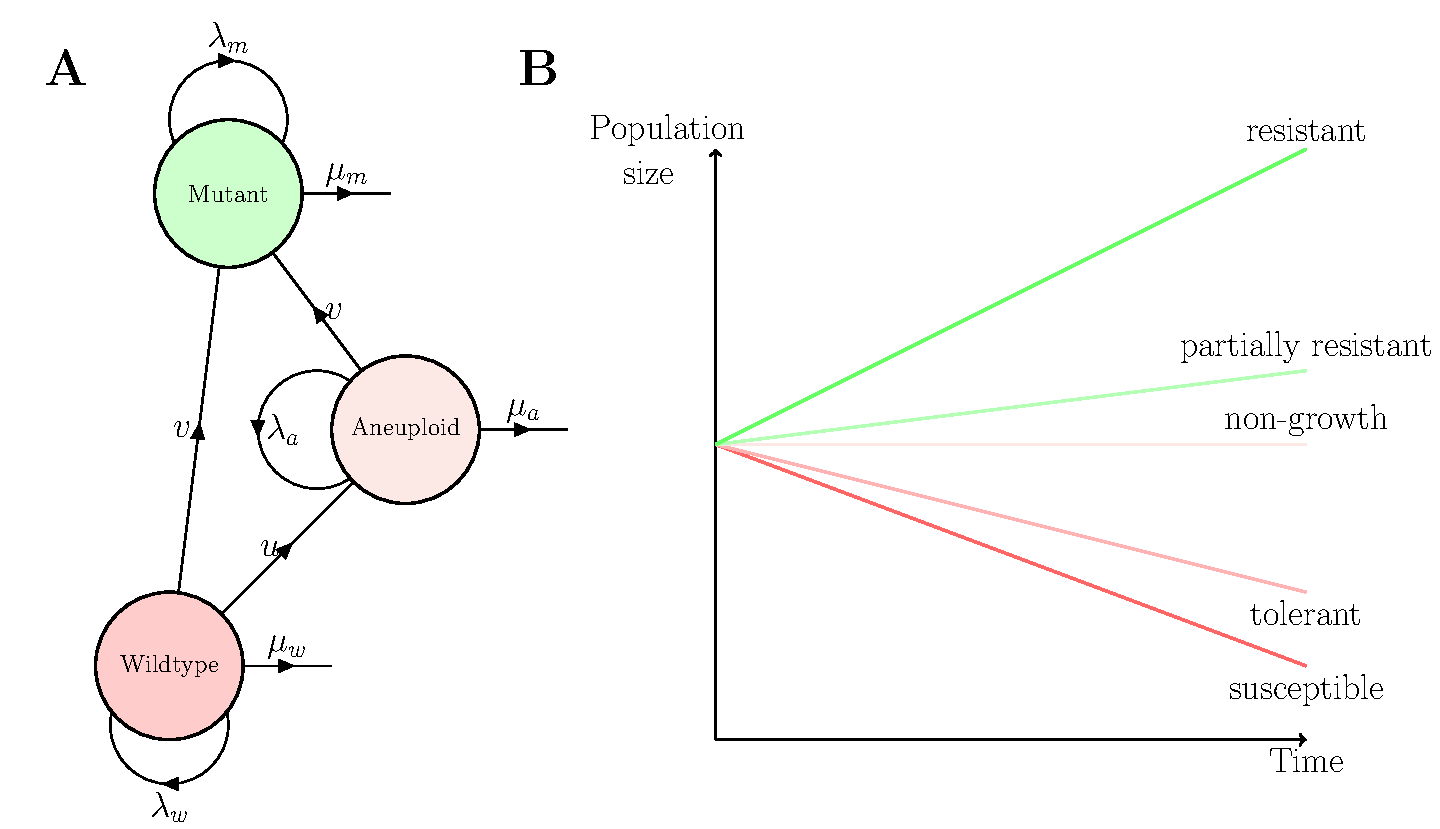
\includegraphics[width=0.75\textwidth]{Figures/figureAneuploidy.pdf}
\caption{
\textbf{Model illustration.}
\textbf{(A)} A population of cancer cells is composed of wildtype, aneuploid, and mutant cells, which divide with rates $\lambda_w$, $\lambda_a$, and $\lambda_m$ and die at rates $\mu_w$, $\mu_a$, and $\mu_m$, respectively. 
Wildtype cells can become aneuploid at rate $u$. Both aneuploid and wildtype cells can acquire a beneficial mutation with rate $v$. Color denotes the relative growth rates of the three genotypes such that $\lambda_w - \mu_w < \lambda_a - \mu_a < \lambda_m - \mu_m$. \textbf{(B)} The wildtype and the mutant are susceptible and resistant, respectively, to the drug. The aneuploid may be tolerant, non-growing, or or partially resistant.
}
\label{figureAneuploidy}
\end{figure}

%%%%%%%%%%%

\begin{figure}
% TODO change panel labels to ABCD
\begin{subfigure}{0.5\textwidth}
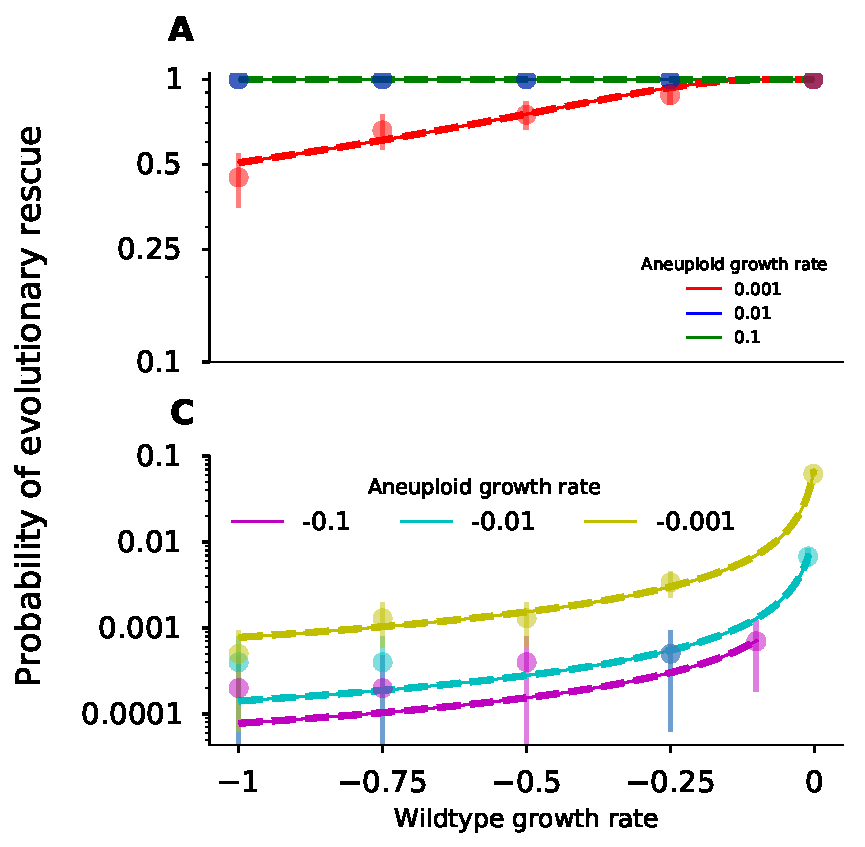
\includegraphics[width=1\textwidth]{Figures/CombinedSubplot.pdf}
\end{subfigure}
\begin{subfigure}{0.5\textwidth}
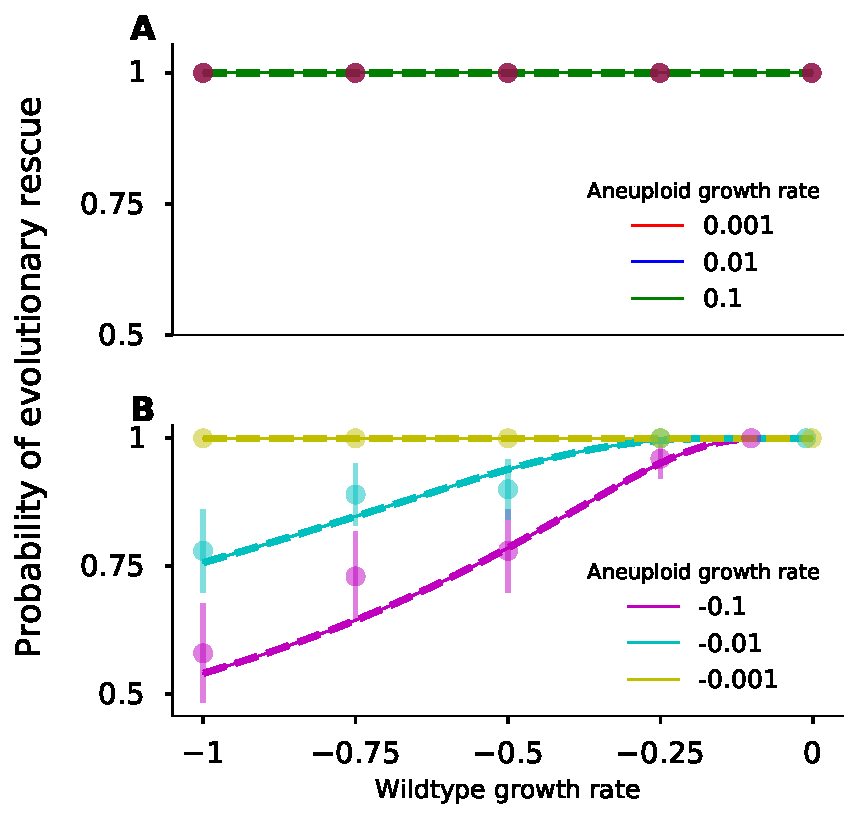
\includegraphics[width=1\textwidth]{Figures/CombinedSubplotLargePop.pdf}
\end{subfigure}
\caption{
\textbf{Evolutionary rescue probability with partially resistant or tolerant aneuploid cells.}
Rescue probability is very high when aneuploidy provides partial resistance ($\lambda_a=0.01$), in an initially small tumor (\textbf{Aleft}, $N=10^4$) and even more so in an initially large tumor (\textbf{Aright}, $N=10^8$). 
When aneuploidy provides tolerance (\textbf{Bleft}, $N=10^4$; \textbf{Bright}, $N=10^8$), the rescue probability is much lower. 
In both scenarios, rescue probability increase with both the wildtype growth rate (x-axis) and the aneuploidy growth rate (colors).
Markers represent simulation results with 95\% CI; solid and dashed lines for the exact formula (\cref{survival_prob} in \cref{rescue_prob}); dashed lines for the approximate formula (\cref{rescue_prob_approx}), demonstrating that they all agree.
Parameters: division rate $\lambda_w=\lambda_a=\lambda_m=0.14$ (so that growth rate changes due to variable death rate); mutant death rate $\mu_m=0.13$ (so that mutant growth rate $\Delta_m=0.01$); aneuploidy rate $u=10^{-2}$; mutation rate $v=10^{-7}$.
}
\label{rescue_prob_wt_growth}
\end{figure}
%%%%%%%%%%%

\begin{figure}
% small population size
% switch from tolerance to non-growing
% TODO why no switch in panel B?
% TODO more simulations for 0 > Delta_a > Delta^*_a
\begin{subfigure}{0.5\textwidth}
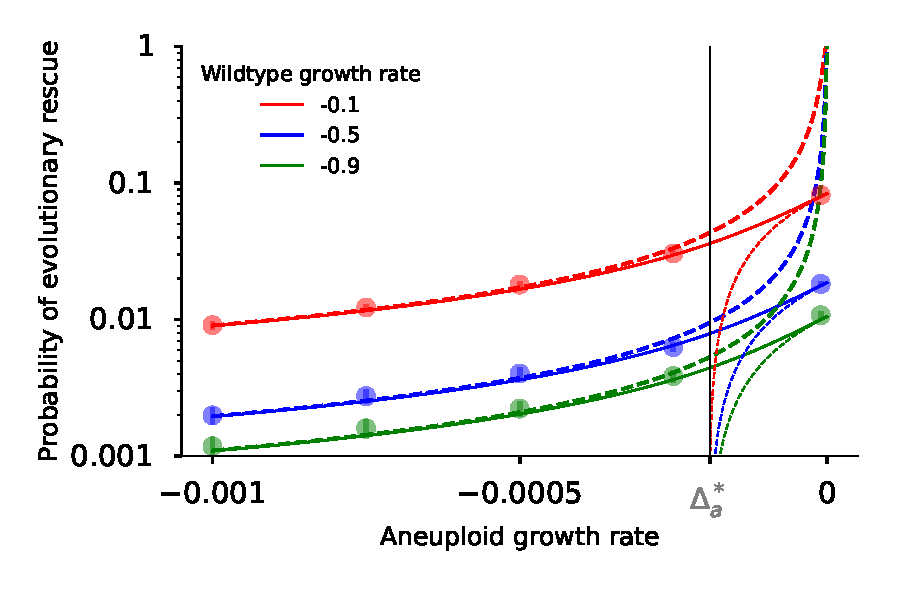
\includegraphics[width=1\textwidth]{Figures/P_est_divergence.pdf}
\end{subfigure}
\begin{subfigure}{0.5\textwidth}
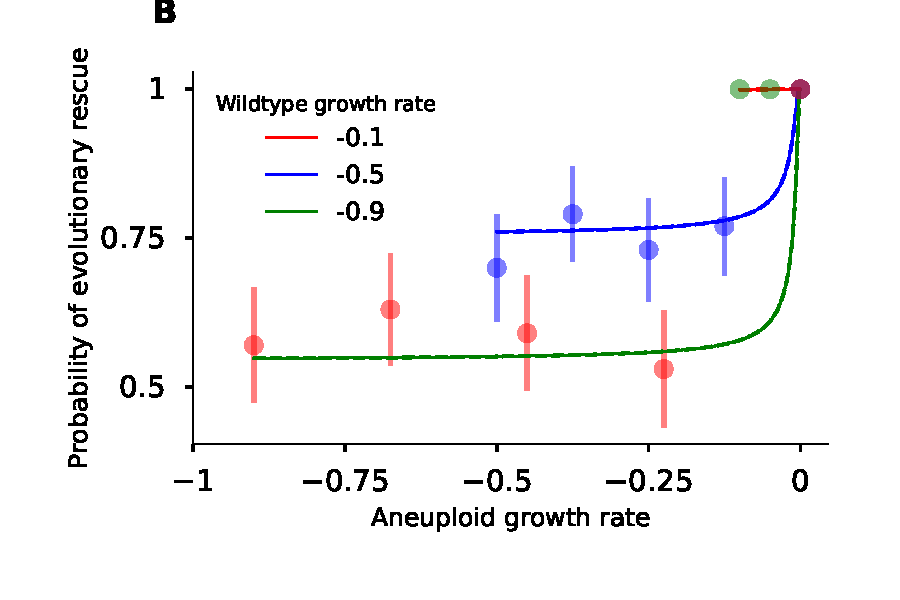
\includegraphics[width=1\textwidth]{Figures/P_est_divergenceLargePopulation.pdf}
\end{subfigure}
\caption{\textbf{Evolutionary rescue probability with tolerant or non-growing aneuploid cells.}
Rescue probability grows with the aneuploid growth rate $\Delta_a$ (x-axis), and is much higher in an initially large tumor than in a small one (\textbf(A) $N=10^4$; \textbf{(B)} $N=10^8$). 
Markers for simulation results with 95\% CI; 
solid lines for the exact formula (\cref{survival_prob} in \cref{rescue_prob});
dashed lines for the approximate formula (\cref{rescue_prob_approx}).
The approximation agrees with the simulation and exact solution when the initial tumor size is large (panel B).
When the tumor size is small (panel A), we switch between the approximation for tolerant and for non-growing aneuploid cells; the switch occurs at $\Delta_a^*=2vp_m+v+2\sqrt{vp_m\left(vp_m+\mu_a+v\right)}$.
Parameters: $\lambda_w=\lambda_a=\lambda_m=0.14$; $\mu_m=0.13$; $u=10^{-2}$; $v=10^{-7}$.
}
\label{rescue_prob_an_growth}
\end{figure}

%%%%%%%%%%%

\begin{figure}
\begin{subfigure}{0.5\textwidth}
% non-growing slightly declining, compare 1st order approximation to exact and simulation
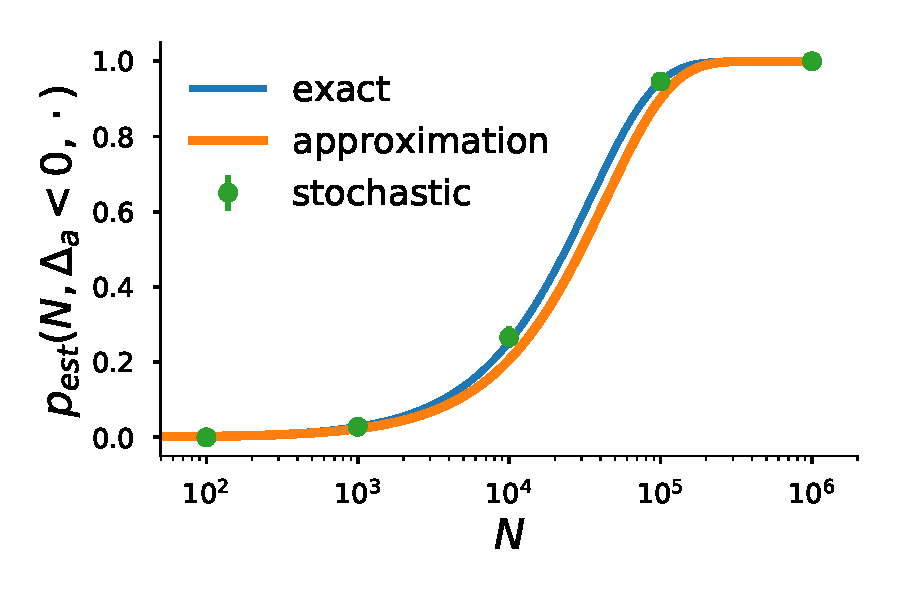
\includegraphics[width=1\textwidth]{Figures/DeleteriousTauLeapPlot.pdf}
\end{subfigure}
\begin{subfigure}{0.5\textwidth}
% density-dependent simulations, barely growing (or maybe partial resistance), with exact formula
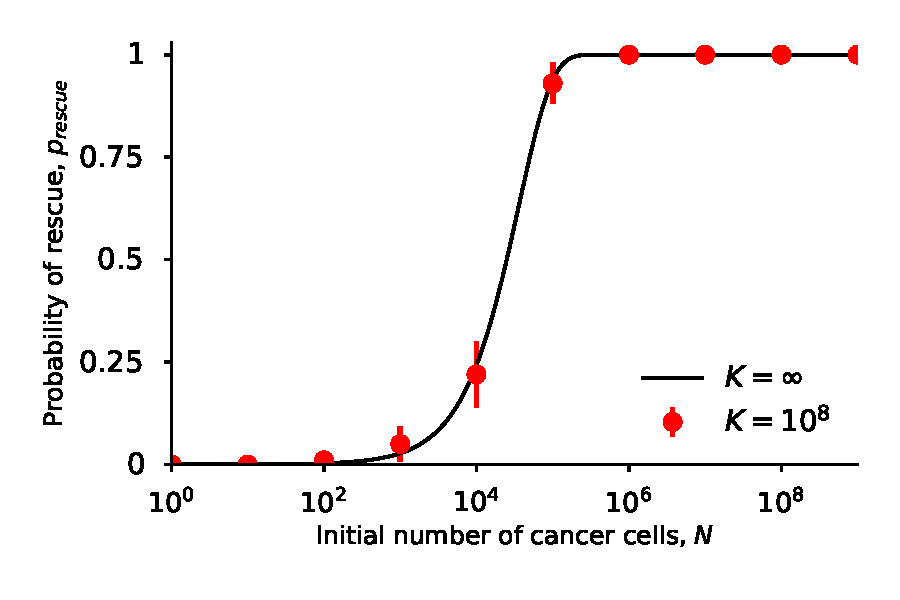
\includegraphics[width=1\textwidth]{Figures/SurvPlotNDataLogisticK.pdf}
\end{subfigure}
\caption{\textbf{Evolutionary rescue probability for variable initial tumor size.}
\textbf{(A)} Comparison of simulation results (markers with 95\% CI, too small to appear with $10^5$ simulations per marker), the exact formula (blue line, \cref{survival_prob} in \cref{rescue_prob}) and the approximate formula (orange line, \cref{rescue_prob_approx}).
\textbf{(B)} Comparison of results of simulations  with density-dependent growth (markers with with 95\% CI) and the exact formula (blue line, \cref{survival_prob} in \cref{rescue_prob}) with maximum carrying capacity $K=10^9$.
Parameters: $\lambda_w=\lambda_a=\lambda_m=0.14$; $\mu_w=0.17$; (A) $\mu_a=0.15$, (B) $\mu_a=0.135$; $\mu_m=0.13$; $u=10^{-2}$; $v=10^{-7}$.
}
\label{rescue_prob_N}
\end{figure}

%%%%%%%%%%%

\begin{figure}
% slightly decreasing (need to check)
 \vspace*{1\baselineskip}
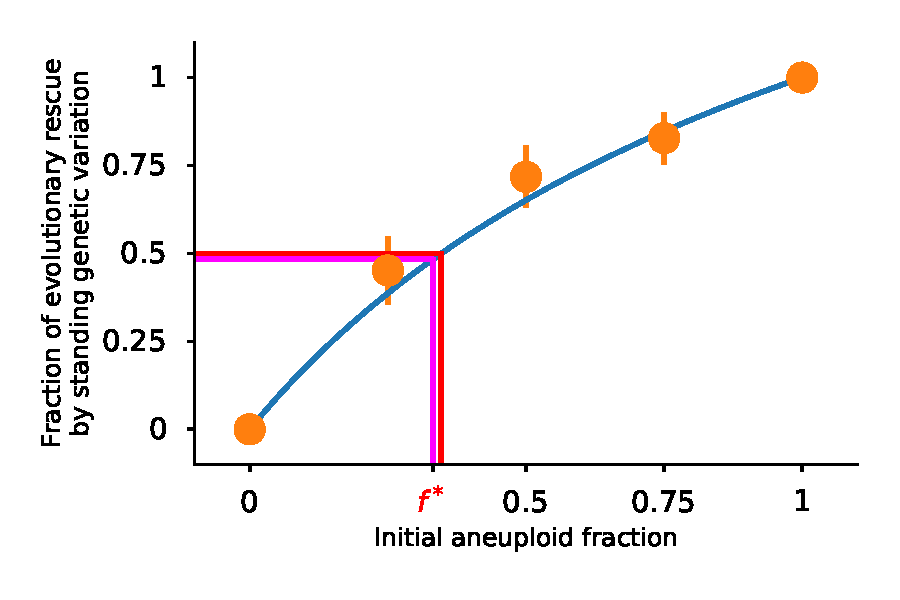
\includegraphics[width=1\textwidth]{Figures/FractionPlot.pdf}
\caption{\textbf{Effect of standing variation on evolutionary rescue.}
In aneuploid cells already exist in the population at the onset of drug therapy as standing genetic variation, then evolutionary rescue is more likely... 
Parameters: $\lambda_w=\lambda_a=\lambda_m=0.14$; $\mu_w=0.17$; $\mu_a=0.145$; $\mu_m=0.13$; $u=10^{-2}$; $v=10^{-7}$.
% TODO think about this figure...
% TODO maybe better to show p_total / p_denovo as function of u or N.
}
\label{FractionPlot}
\end{figure}

%%%%%%%%%%%

\begin{figure}
% A partial resistance
% B tolerance
% left function of wildtype growth rate 
% right function of population size
\begin{subfigure}{0.5\textwidth}
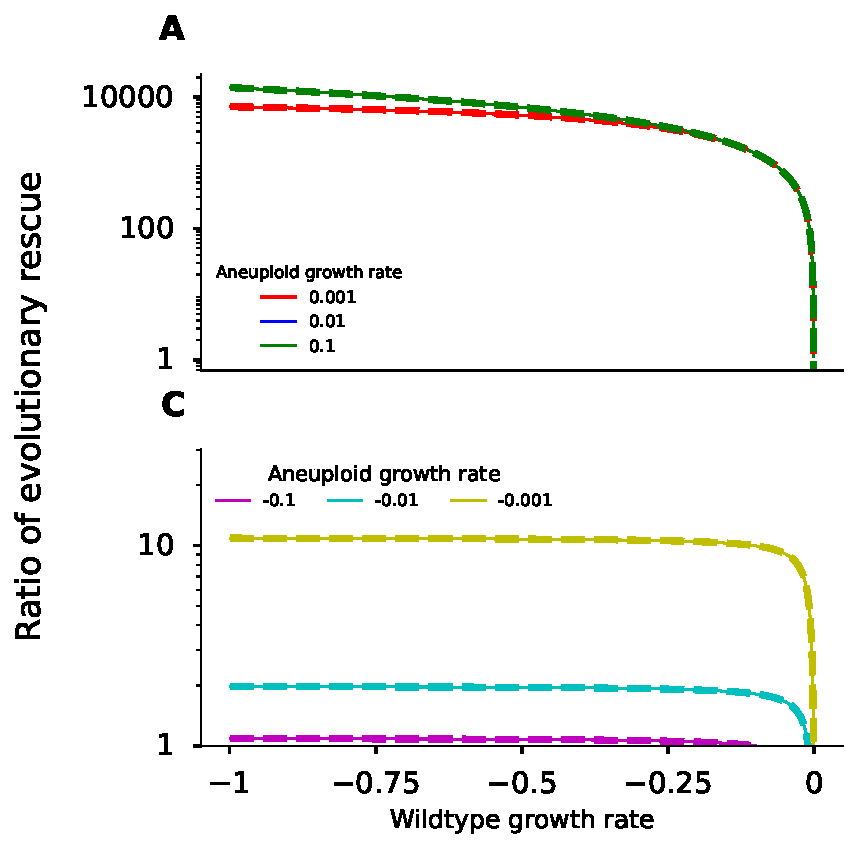
\includegraphics[width=1\textwidth]{Figures/RatioEvolRescue.pdf}
\end{subfigure}
\begin{subfigure}{0.5\textwidth}
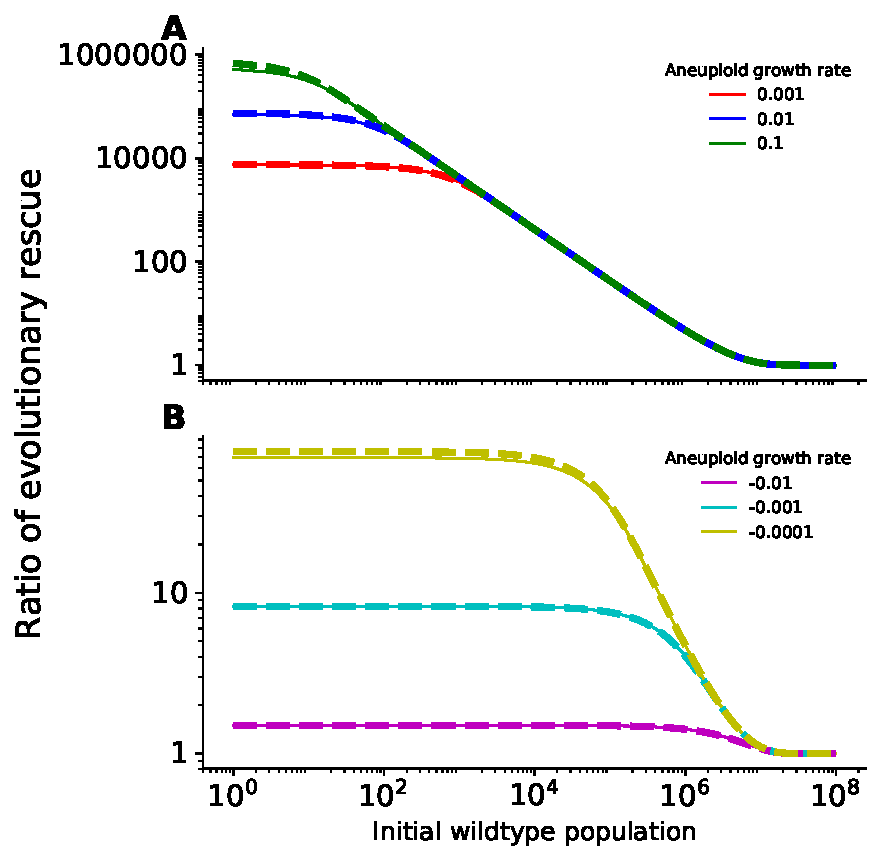
\includegraphics[width=1\textwidth]{Figures/RatioEvolRescuePopulationSize.pdf}
\end{subfigure}
\caption{\textbf{Effect of aneuploidy on evolutionary rescue.}
The ratio of rescue probability with and without aneuploid ($H$, \cref{ratiorescue}) increases with the aneuploid growth rate (colors) and decreases with the wildtype growth rates and initial tumor size (x-axes), except for large tumors where where the ratio converges to unity.
\textbf{(A-left,A-right)} Aneuploidy provides partial resistance.
\textbf{(B-left, B-right)} Aneuploidy provides tolerance.  
Solid and dashed lines apply $p_{rescue}$ from the exact formula of  (\cref{survival_prob} in \cref{rescue_prob}); dashed lines apply $p_{rescue}$ from the approximate formula (\cref{rescue_prob_approx}), with good agreement.
Parameters: $N=10^4$; $\lambda_w=\lambda_a=\lambda_m=0.14$; (B) $\mu_w=0.17$; $\mu_m=0.13$; $u=10^{-2}$; $v=10^{-7}$.
% TODO start y at 1
% TODO fix panel labels
}
\label{rescue_ratio}
\end{figure}

%%%%%%%%%%%

\begin{figure}
\begin{subfigure}{0.5\textwidth}
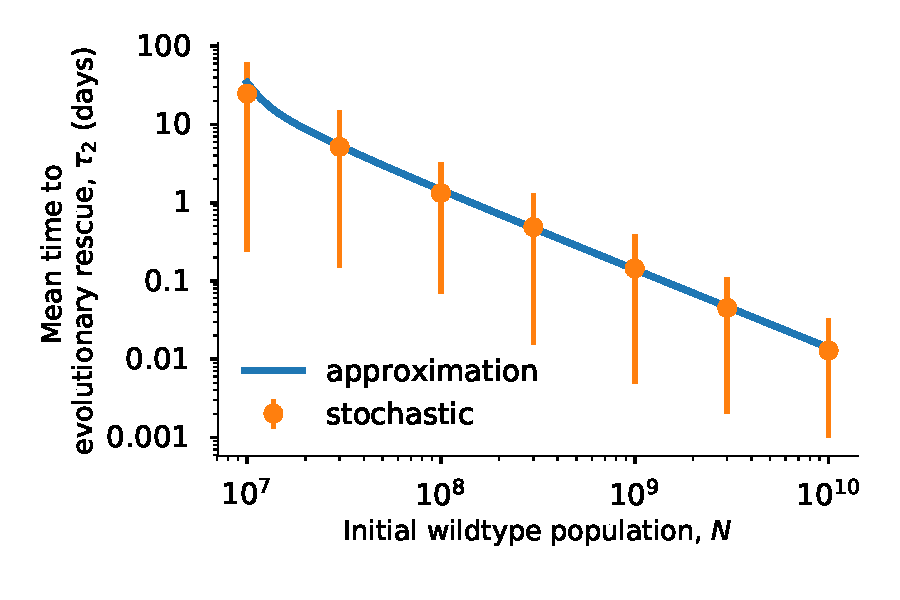
\includegraphics[width=1\textwidth]{Figures/MeanTimeDeleteriousPlot.pdf}
\end{subfigure}
\begin{subfigure}{0.5\textwidth}
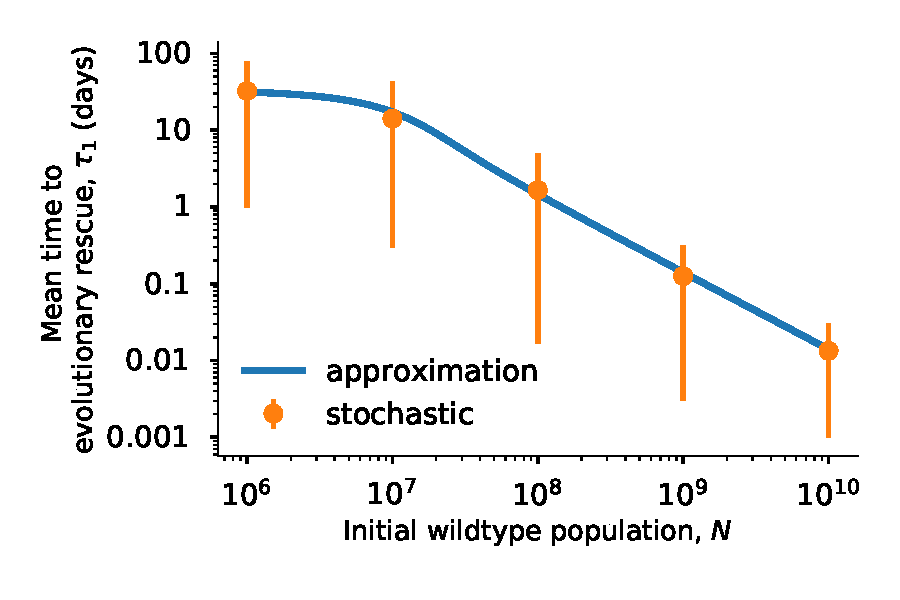
\includegraphics[width=1\textwidth]{Figures/MeanTimeGrowthMutantDirectPlot.pdf}
\end{subfigure}
\caption{\textbf{Evolutionary rescue time.}
Shown is the mean time for appearance of a resistance mutation the leads to evolutionary rescue \textbf{(left)} with ($u>0$) and \textbf{(right)} without ($u=0$ aneuploidy.
Our inhomogeneous Poisson-process approximations (solid blue lines, right: \cref{meantime1}, left: \cref{meantimet2}) is in agreement with simulation results (orange markers with 95\% CI).
Our 1st-order (dashed red lines, right: \cref{limitapprox}, left: \cref{limitapprox2}) and 2nd-order (green line, left: \cref{limitapprox3}) approximations work well when the initial tumor size is large (here $>10^8$ cells).
Parameters: $\lambda_w=\lambda_a=\lambda_m=0.14$; $\mu_w=0.17$; (A) $\mu_a=0.145$; $\mu_m=0.13$; $u=10^{-2}$; $v=10^{-7}$.
}
\label{MeanTimeGrowthAneuploidyPlot} 
\end{figure}

%%%%%%%%%%%

\begin{figure}
% tolerance... maybe third is slightly decreasing
 \vspace*{1\baselineskip}
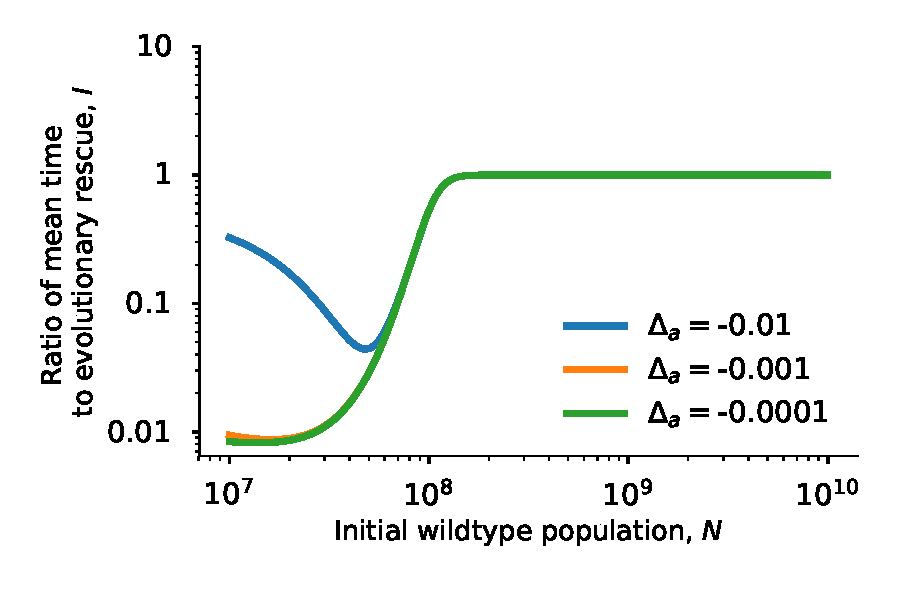
\includegraphics[width=1\textwidth]{Figures/MeanTimeRatioInitialPopulationSize.pdf}
\caption{\textbf{Ratio of evolutionary rescue time with and without aneuploidy.}
The ratio of the mean time to appearance of a resistance mutation that leads to evolutionary rescue with ($u>0$) and without ($u=0$) aneuploidy for variable initial tumor sizes (\cref{eqMeanTimeRatioInitialPopulationSize}) when aneuploidy provides tolerance to the drug ($\Delta_a\ll0$). When the initial tumor size is not large ($<10^8$), aneuploidy can decrease the rescue time by 10-100-fold.
\emph{I THINK THERE IS A MISTAKE IN THE BLUE LINE} % TODO
% TODO parameter values 
}
\label{MeanTimeRatioInitialPopulationSize}
\end{figure}

%%%%%%%%%%
%
%\begin{figure}
%% diffusion approx instead of branching process
%% tolerance
% \vspace*{1\baselineskip}
%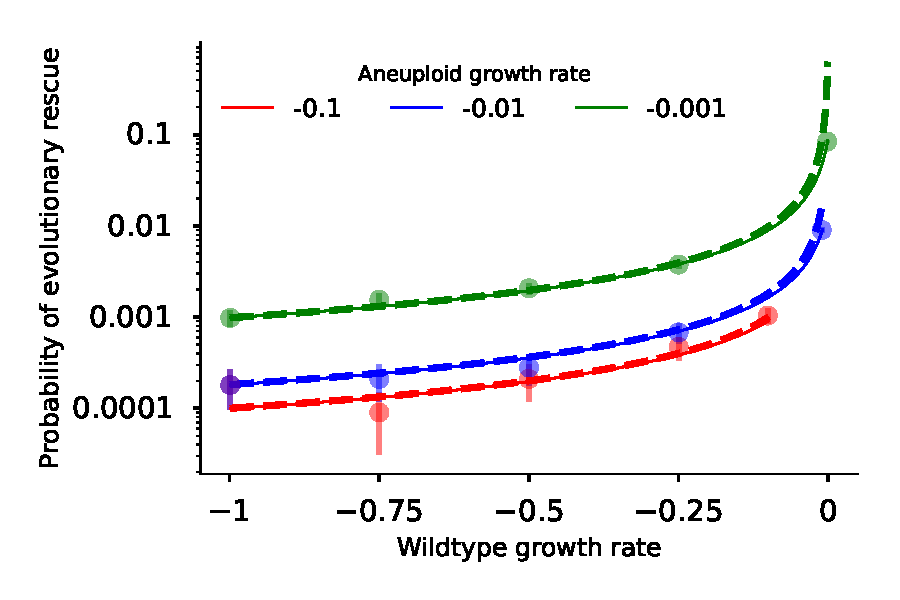
\includegraphics[width=1\textwidth]{Figures/P_est_diffusion.pdf}
%\caption{Plot of the survival probability of an initial population consisting of $w_0=10^{4}$ wildtype cells as a function of $\Delta_a=\lambda_a-\mu_a$ for various values of $\Delta_w=\lambda_a-\mu_a$. The continuous lines represent the exact result \eqref{survprobw} while the dashed lines represent the Feller diffusion approximation \eqref{FellerApprox}. The error bars represent $95\%$ confidence interval of the form $p\pm1.96\sqrt{p\left(1-p\right)/w_0}$ where $p$ is the mean probability of evolutionary rescue.}
%\label{P_est_diffusion}
%\end{figure}
%
%%%%%%%%%%%
%
%\begin{figure}
%% partial resistance, compare 1st and 2nd order approximation and exact
%\vspace*{1\baselineskip}
%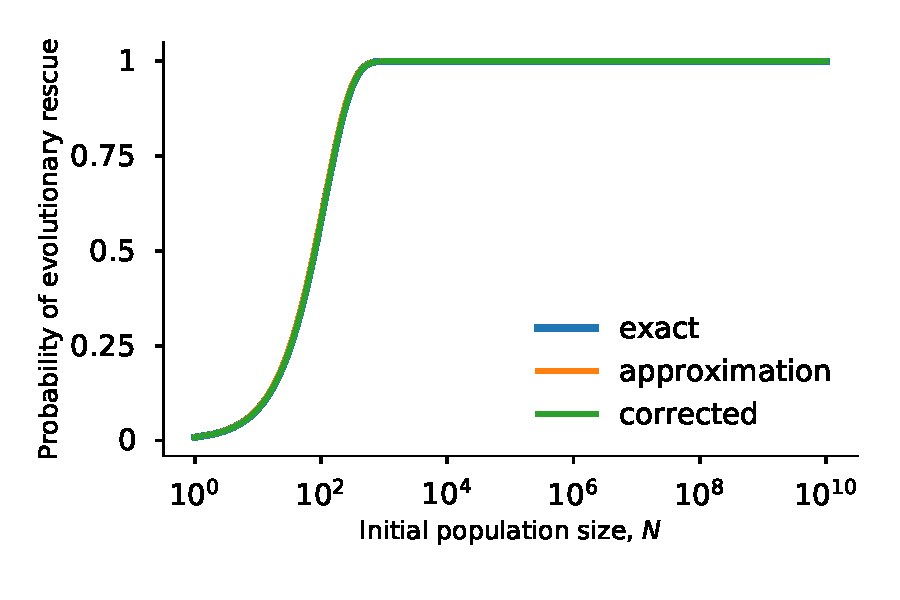
\includegraphics[width=1\textwidth]{Figures/SurvPlotNData.pdf}
%\caption{Plot of the probability of survival of a population as a function of the initial population size of wildtype cells. The blue line represents the exact solution \eqref{survprobw}, the orange line line represents the approximation \eqref{aneuploidyresistentfirstapprox}, the green line represents the first order correction \eqref{survprobwapproxcorrected} and the red dots represents stochastic simulations. For the simulations we have chosen the following parameters: $\lambda_w=0.14, \lambda_a=0.14,\lambda_m=0.14,\mu_w=0.17,\mu_a=0.135,\mu_m=0.13$. The error bars represent $95\%$ confidence interval of the form $p\pm1.96\sqrt{p\left(1-p\right)/n}$ where $p$ is the mean probability of evolutionary rescue and $n=100$ is the number of simulations.}
%\label{compare_1st_2nd_order_approx}
%\end{figure}

%%%%%%%%%%%%%%%%%%%%%%%%%%%%%%%%%%%%%%%%%%

%\appendix
%\begin{appendices}
%\renewcommand{\theequation}{\thesection\arabic{equation}}
%\counterwithin*{equation}{section}

%%%%%%%%%%%%%%%%%%%%%%%%%%%%%%%%%%%%%%%%%%
%\section*{Gillespie algorithm}
%\begin{subequations}
%\begin{flalign}
%(+1,0,0)&:\quad \lambda_ww_t,\\
%(-1,0,0)&:\quad \mu_ww_t,\\
%(-1,+1,0)&:\quad uw_t,\\
%(-1,0,+1)&:\quad vw_t,\\
%(0,+1,0)&:\quad \lambda_aa_t,\\
%(0,-1,0)&:\quad \mu_aa_t,\\
%(0,-1,+1)&:\quad va_t,\\
%(0,0,+1)&:\quad \lambda_am_t,\\
%(0,0,-1)&:\quad \mu_am_t.
%\end{flalign}
%\end{subequations}

%%%%%%%%%%%%%%%%%%%%%%%%%%%%%%%%%%%%%%%%%%
%%%%%%%%%%%%%%%%%%%%%%%%%%%%%%%%%%%%%%%%%%
%\section*{Mean time}
%%%%%%%%%%%%%%%%%%%%%%%%%%%%%%%%%%%%%%%%%%%
%We define the following events
%\begin{align*}
%\text{EvR}&=\text{``evolutionary rescue occurs''},\\
%\text{EvRA}&=\text{``evolutionary rescue occurs through aneuploidy''},\\
%\text{EvRM}&=\text{``evolutionary rescue occurs through mutation''}.
%\end{align*}
%As a result, the mean time to appearence of the first mutant cell which rescues the population given evolutionary rescue can be expanded as:
%\begin{align*}
%\mathbb{E}\left[\tau|\text{EvR}\right]&=\mathbb{E}\left[\tau|\text{EvR},\text{EvRA}\cap\text{EvRM}^{C}\right]p\left(\text{EvRA}\cap\text{EvRM}^{C}|\text{EvR}\right)\\
%&+\mathbb{E}\left[\tau|\text{EvR},\text{EvRM}\cap\text{EvRA}^{C}\right]p\left(\text{EvRM}\cap\text{EvRA}^{C}|\text{EvR}\right)\\
%&+\mathbb{E}\left[\tau|\text{EvR},\text{EvRM}\cap\text{EvRA}\right]p\left(\text{EvRM}\cap\text{EvRA}|\text{EvR}\right).
%\end{align*}
%The joint probabilities in the previous lines can be written as:
%\begin{align*}
%p\left(\text{EvRA}\cap\text{EvRM}^{C}|\text{EvR}\right)&=\frac{p\left(\text{EvRA}\cap\text{EvRM}^{C}\right)}{p\left(\text{EvR}\right)}
%\approx\frac{p\left(\text{EvRA}\right)\left[1-p\left(\text{EvRM}\right)\right]}{p\left(\text{EvR}\right)},\\
%p\left(\text{EvRM}\cap\text{EvRA}^{C}|\text{EvR}\right)&=\frac{p\left(\text{EvRM}\cap\text{EvRA}^{C}\right)}{p\left(\text{EvR}\right)}
%\approx\frac{p\left(\text{EvRM}\right)\left[1-p\left(\text{EvRA}\right)\right]}{p\left(\text{EvR}\right)},\\
%p\left(\text{EvRM}\cap\text{EvRA}|\text{EvR}\right)&=\frac{p\left(\text{EvRM}\cap\text{EvRA}\right)}{p\left(\text{EvR}\right)}\approx\frac{p\left(\text{EvRM}\right)p\left(\text{EvRA}\right)}{p\left(\text{EvR}\right)}\ll1.
%\end{align*}
%As a result, we have:
%\begin{align*}
%\mathbb{E}\left[\tau|\text{EvR}\right]&\approx\mathbb{E}\left[\tau|\text{EvR},\text{EvRA}\cap\text{EvRM}^{C}\right]p\left(\text{EvRA}\cap\text{EvRM}^{C}|\text{EvR}\right)\\
%&+\mathbb{E}\left[\tau|\text{EvR},\text{EvRM}\cap\text{EvRA}^{C}\right]p\left(\text{EvRM}\cap\text{EvRA}^{C}|\text{EvR}\right).
%\end{align*}
%%%
%%%%%%%%%%%%%%%%%%%%%%%%%%%%%%%%%%%%%%%%%%
%\section*{Diffusion approximation}\label{AppendixDiffApprox}
%
%An alternative method to obtain the probability of evolutionary rescue is to utilize a Feller diffusion approximation which is governed by two parameters: the growth rate $r$ and the reproductive variance $\sigma$. The two parameters are obtained from the underlying demographic process as the infinitesimal relative change in mean and variance of $n_t$ over and an infinitesimally small time interval $\Delta t$:
%\begin{align*}
%r&=\lim_{\Delta t\rightarrow0}\frac{\mathbb{E}\left(\Delta n_t|n_t\right)}{\Delta_t n_t},\\
%\sigma&=\lim_{\Delta t\rightarrow0}\frac{\mathbb{V}ar\left(\Delta n_t|n_t\right)}{\Delta_t n_t}.
%\end{align*}
%The rate at which mutants are generated directly from the wildtype is: 
%\begin{align}
%\theta_1=v\bar{\pi}_f\frac{N}{|r_w|},
%\end{align}
%where
%\begin{align}
%\bar{\pi}_f=\int_{0}^\infty\int_{0}^\infty \left(1-\e^{-\frac{2r}{\sigma}}\right) f_r\left(r,\sigma\right)\d r\d\sigma.
%\end{align}
%Letting $f_r\left(r,\sigma\right)=\delta\left(r-r_m\right)\delta\left(\sigma-\sigma_m\right)$ then:
%\begin{align}
%\bar{\pi}_f=1-\e^{-\frac{2r_m}{\sigma_m}},
%\end{align}
%and, as a result, we have:
%\begin{align}
%\theta_1=v\left(1-\e^{-\frac{2r_m}{\sigma_m}}\right)\frac{N}{|\Delta_w|}.
%\end{align}
%The rate at which mutants are generated indirectly from the wildtype through aneuploidy is: 
%\begin{align*}
%\theta_2&=\frac{uN}{|r_w|}\int_{0}^\infty\int_{0}^\infty \left(1-\pi_f\left(r,q\right)\right) f_r\left(r,\sigma\right) p_1^*\left(r,\sigma\right)\d r\d\sigma\\
%&=\frac{uN}{|\Delta_w|}p_1^*\left(r_a,\sigma_a\right)\\
%&=\frac{uN}{|\Delta_w|}\left[1-\exp\left(-\frac{|r_a|}{\sigma_a^2}\left(\sqrt{1+\frac{2\sigma_a^2}{r_a^2}u^*}-1\right)\right)\right]\\
%&=\frac{uN}{|\Delta_w|}\left[1-\exp\left(-\frac{|\Delta_a|}{(\lambda_a+\mu_a)^2}\left(\sqrt{1+\frac{2(\lambda_a+\mu_a)^2}{\Delta_a^2}u^*}-1\right)\right)\right],
%\end{align*}
%where
%\begin{equation}
%u^*=v\left(1-\e^{-\frac{2r_m}{\sigma_m}}\right).
%\end{equation}
%The number of rescue mutations has a Poisson distribution with rate $\theta_1+\theta_2$. As a result, the probability of evolutionary rescue is given by:
%\begin{equation}\label{FellerApprox}
%p_{rescue}=1-\e^{-\left(\theta_1+\theta_2\right)},
%\end{equation}
%which we plot in Figure \ref{P_est_diffusion} as a function of $\Delta_w$.


%\end{appendices}

%%%%%%%%%%%%%%%%%%%%%%%%%%%%%%%%%%%%%%%%%%
\end{document}